\begin{refsection}

\chapter{Experimental methods}
As mentioned above, X- and Ch-bonded interactions were originally identified crystallographically, with additional spectroscopic evidence being present.
These pioneering methods have not changed a great deal, and x-ray crystallography is still the most powerful tool we have to study these interactions.
We also use a number of spectroscopic and computational techniques to probe the nature of Ch-bonding.
Some of the methods used in this thesis are explained below.

\section{Computational methods}
Computational methods are an indispensable tool for chemists, allowing us to study molecules too fragile to isolate in the laboratory, and extract further insight from real-world systems.
A number of the techniques used in this thesis are briefly explained below.

\subsection{Natural Bond Orbital theory}
The SCF procedure, which is at the heart of almost all quantum chemistry calculations, affords a solution wave function $ \Psi $ to the Schr\"{o}dinger equation (\cref{eqn:schrodinger}).

\begin{equation}
    \hat{\mathrm{H}}\Psi = E\Psi
    \label{eqn:schrodinger}
\end{equation}

Within Hartree-Fock theory, the wave function $ \Psi $ is approximated by a single Slater determinant, which is an combination of one electron wave functions $\chi_{n}(\mathbf{x}_{n})$.
Each one electron wave function, or molecular orbital (MO), describes the distribution of an electron in the field of the nuclear potentials, and is generally constructed from a Linear Combination of Atomic Orbitals (LCAO)\footnote{An alternative approach is that of plane-wave basis sets, which are better suited to infinitely periodic systems.}, that is, sums and differences of atom centred basis functions of various symmetries.
The Pauli exclusion principle states that a (many-particle) wave function must be antisymmetric with respect to exchange of two fermionic particles such as electrons, and this requirement is satisfied by the use of a Slater determinant.
This means that for every MO resulting from the sum of two atomic orbitals, there must be a corresponding MO resulting from the difference of the same two atomic orbitals, from which we obtain the familiar MO construction for simple diatomics (\cref{fig:h-orbital-diagram}).

\begin{figure}
    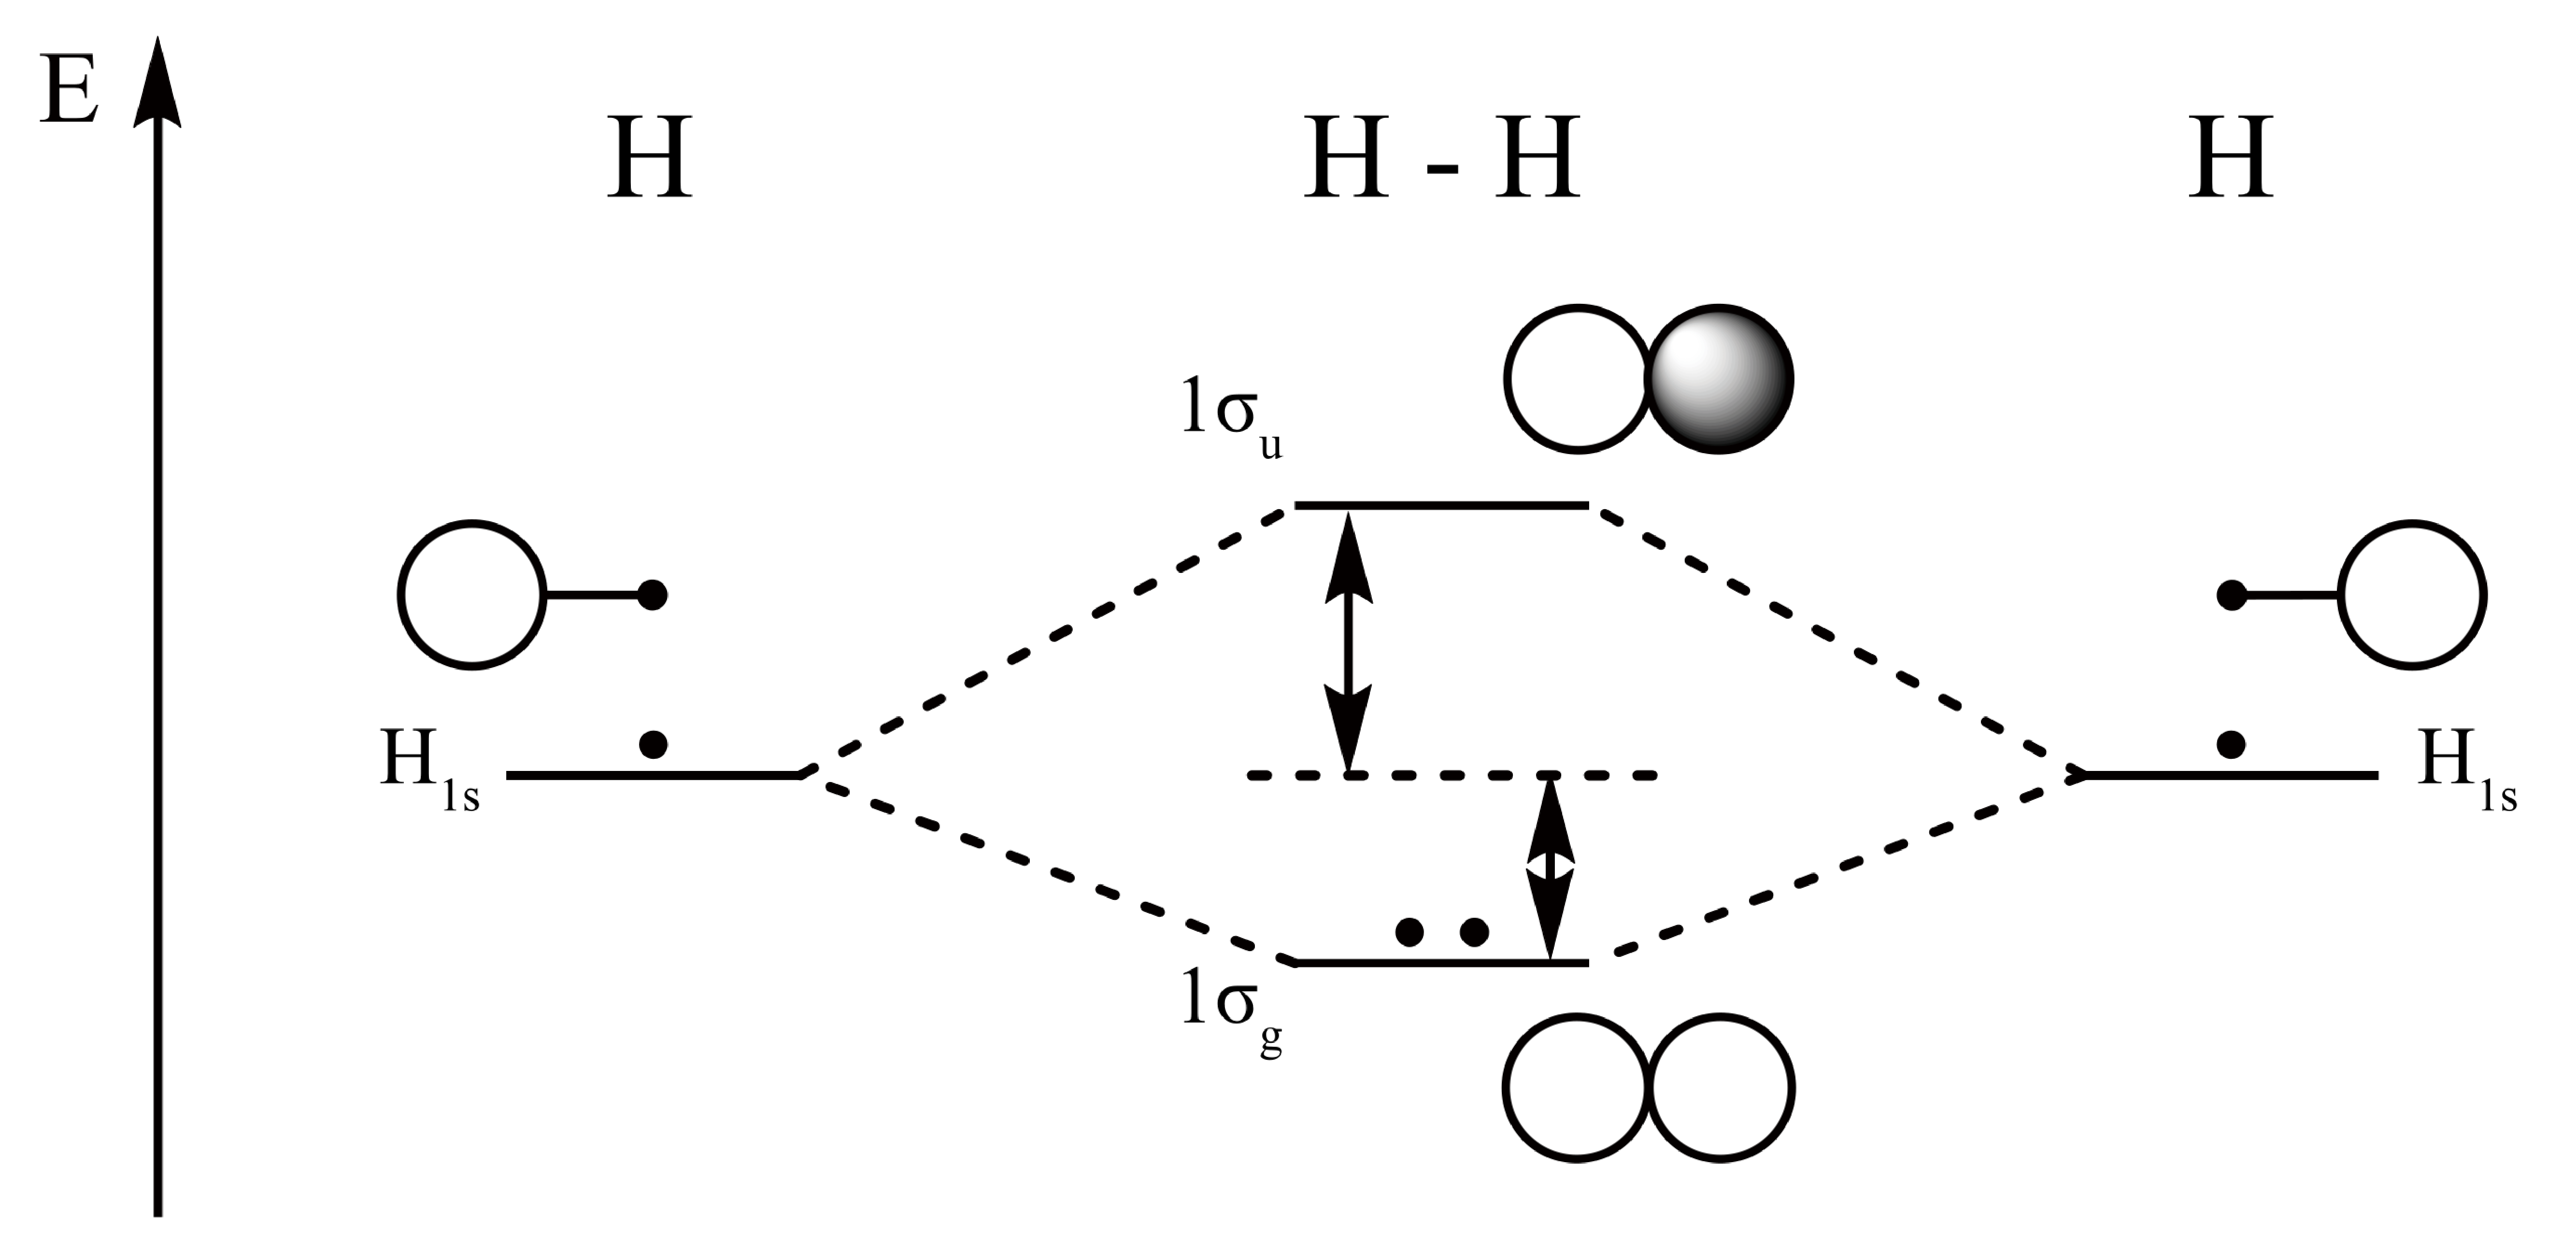
\includegraphics[width=0.6\linewidth]{Figures/h-orbital-diagram.pdf}
    \caption[MO diagram for dihydrogen.]{MO diagram for dihydrogen. Reproduced from reference~\cite{h-orbital-diagram}.}\label{fig:h-orbital-diagram}
\end{figure}

In more complex polyatomic species, these MOs are most easily interpreted as eigenfunctions of the molecular Hamiltonian, and their energies are the corresponding eigenvalues. 
These orbitals describe the distribution of each electron throughout the molecule and hence the bonding within the molecule, but do not translate well into the more intuitive valence bond description of bonding that is most useful to chemists.
From a series of MOs, there is not an easy way to draw a Lewis structure of the molecule at hand.
This is because MOs tend to be highly delocalised throughout the molecule, which is obvious even in the relatively simple case of benzene (\cref{fig:benzene-mo}).

\begin{figure}
    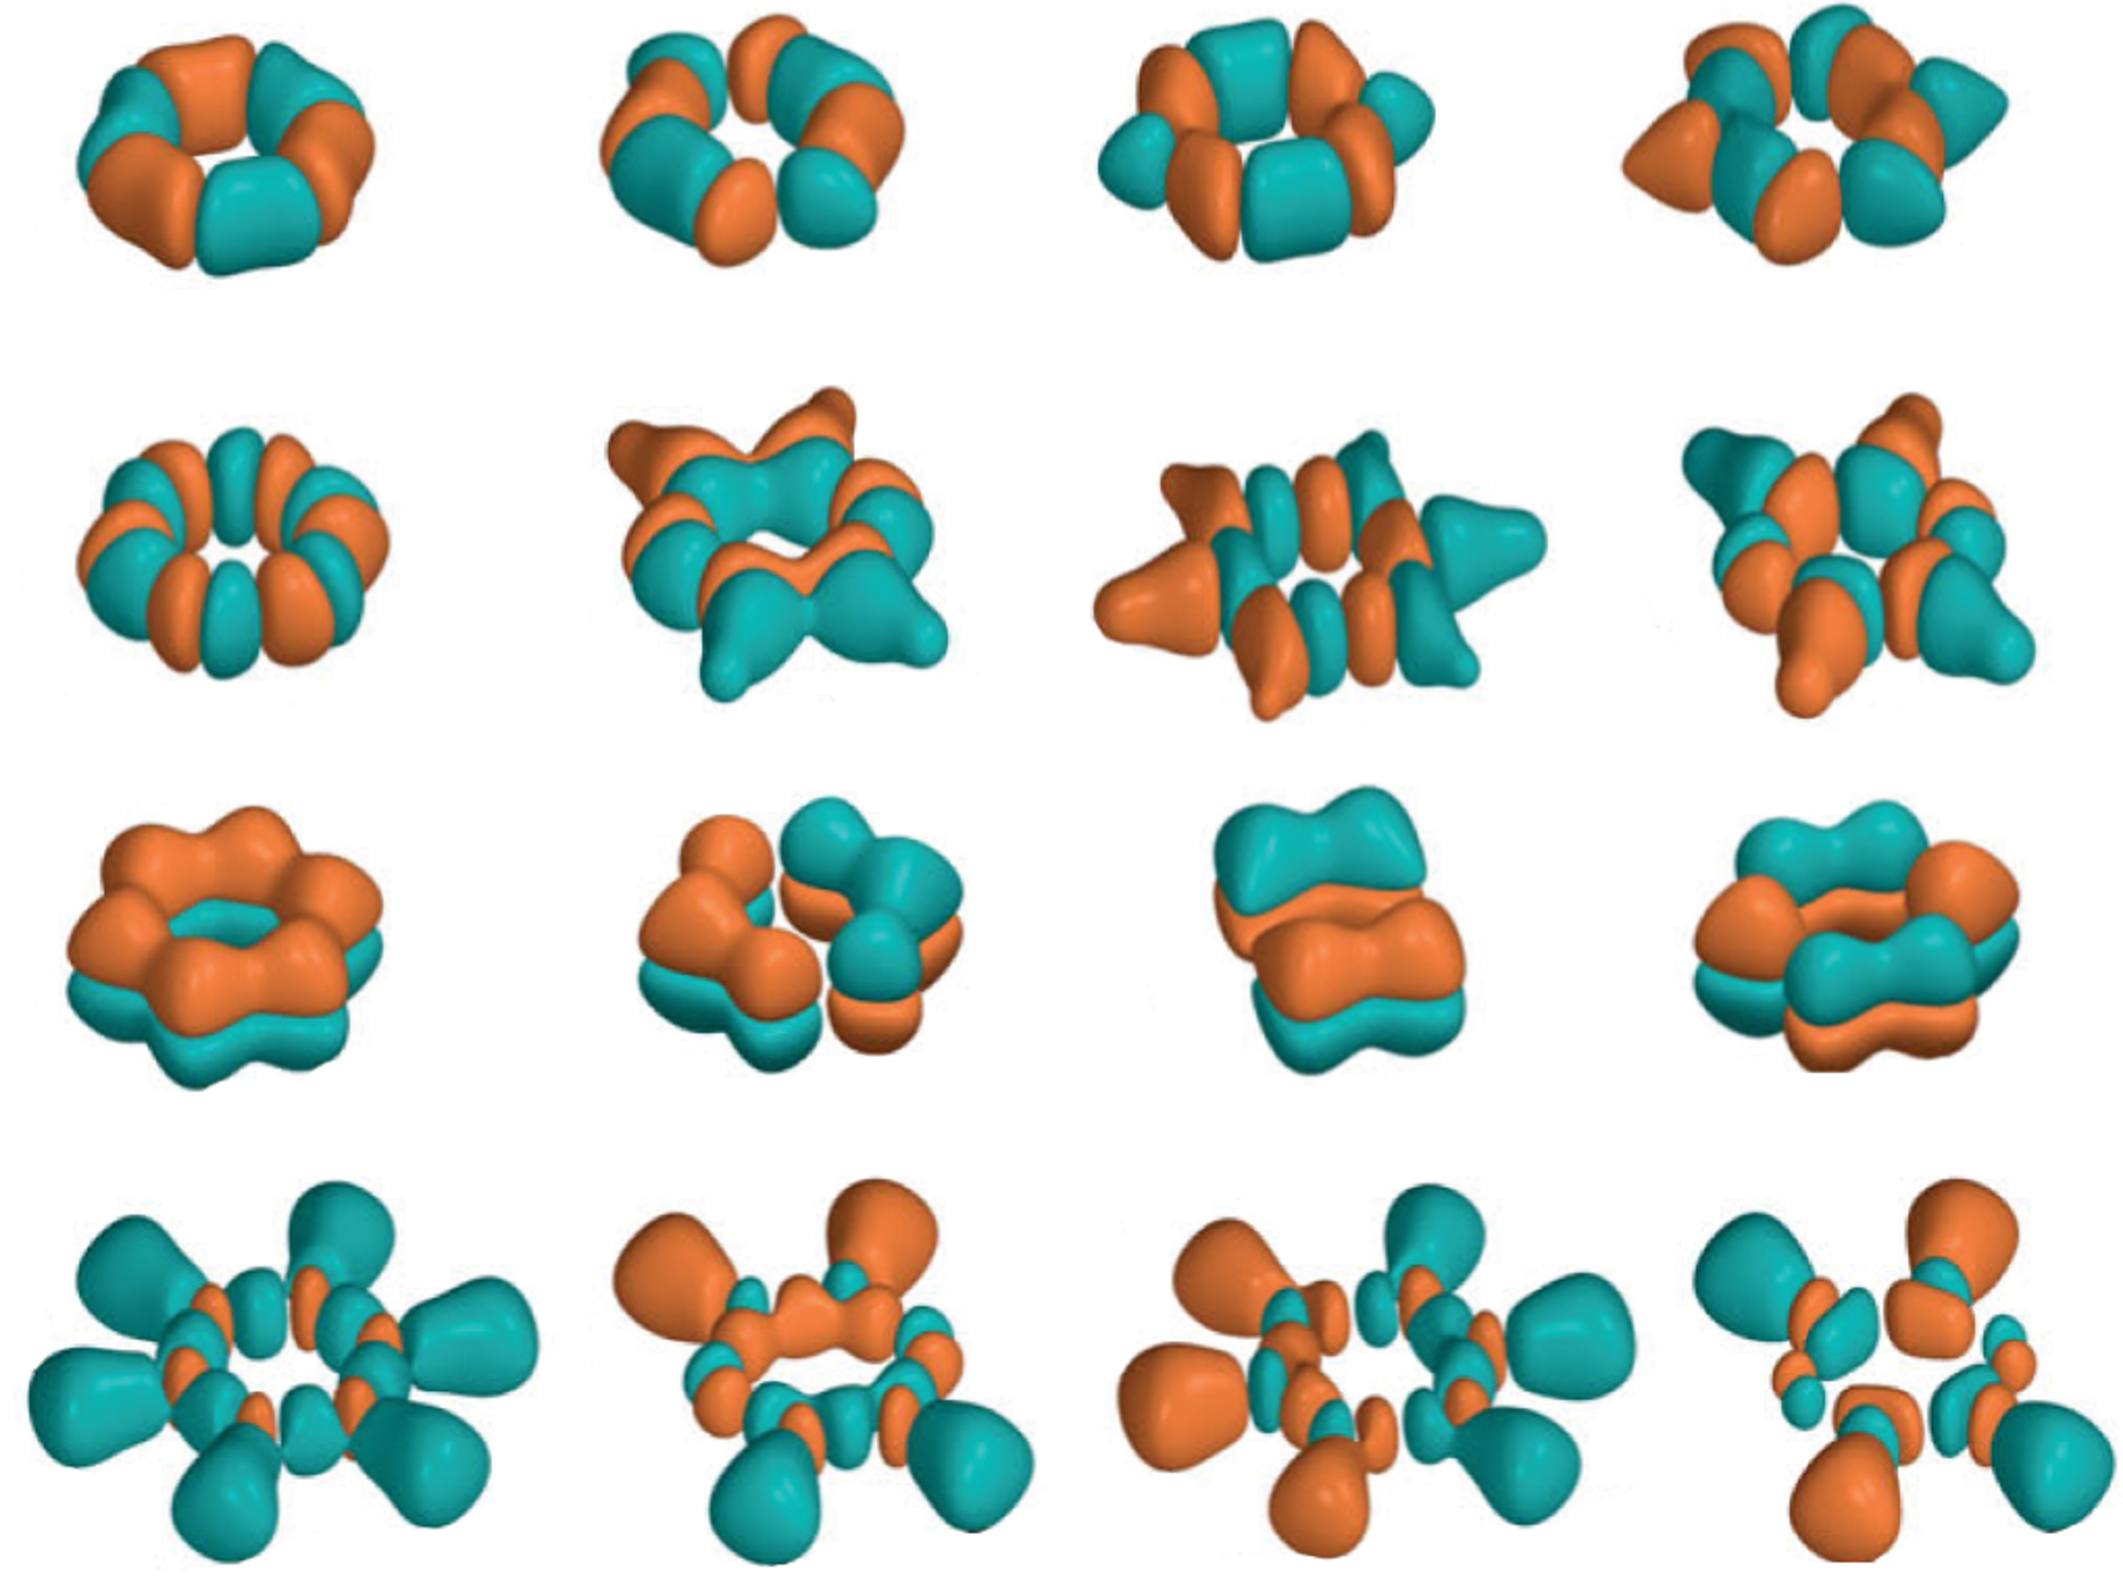
\includegraphics[width=0.8\linewidth]{Figures/benzene-mo.pdf}
    \caption[Molecular orbitals of benzene.]{Molecular orbitals of benzene. Reproduced from reference~\cite{Luhmann2015}.}\label{fig:benzene-mo}
\end{figure}

The Natural Bond Orbital (NBO) scheme attempts to ameliorate this delocalisation, by transforming the molecular orbitals into NBOs which correspond to features found in a Lewis structure.\autocite{Reed1988}
These take the form of one centre and two centre elements (lone pairs and bonding orbitals respectively), which together form the optimal Lewis structure for a molecule.
The NBO scheme also provides a framework for non-Lewis features, such as non-valence electrons which are found in core NBOs.
As a consequence of the transformation from atomic orbitals to NBOs, higher energy two centre elements arise, which correspond to anti-bonding orbitals whose partial occupancy leads to reduction of bond order.
Rydberg NBOs complete the span of the NBO space, which are high energy, highly diffuse orbitals which typically contribute little to the overall chemistry of the system. 
Examples of NBOs in a simple molecule are shown in \cref{fig:nbos}

\begin{figure}
    \centering
    \begin{subfigure}{0.3\linewidth}
        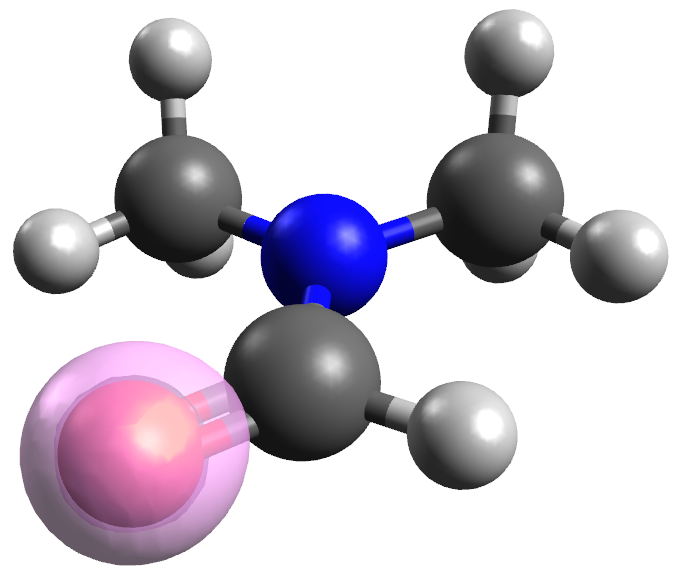
\includegraphics[width=\linewidth]{Figures/dmfnbo-core.png}
        \caption{Core NBO.}
    \end{subfigure}
    \begin{subfigure}{0.3\linewidth}
        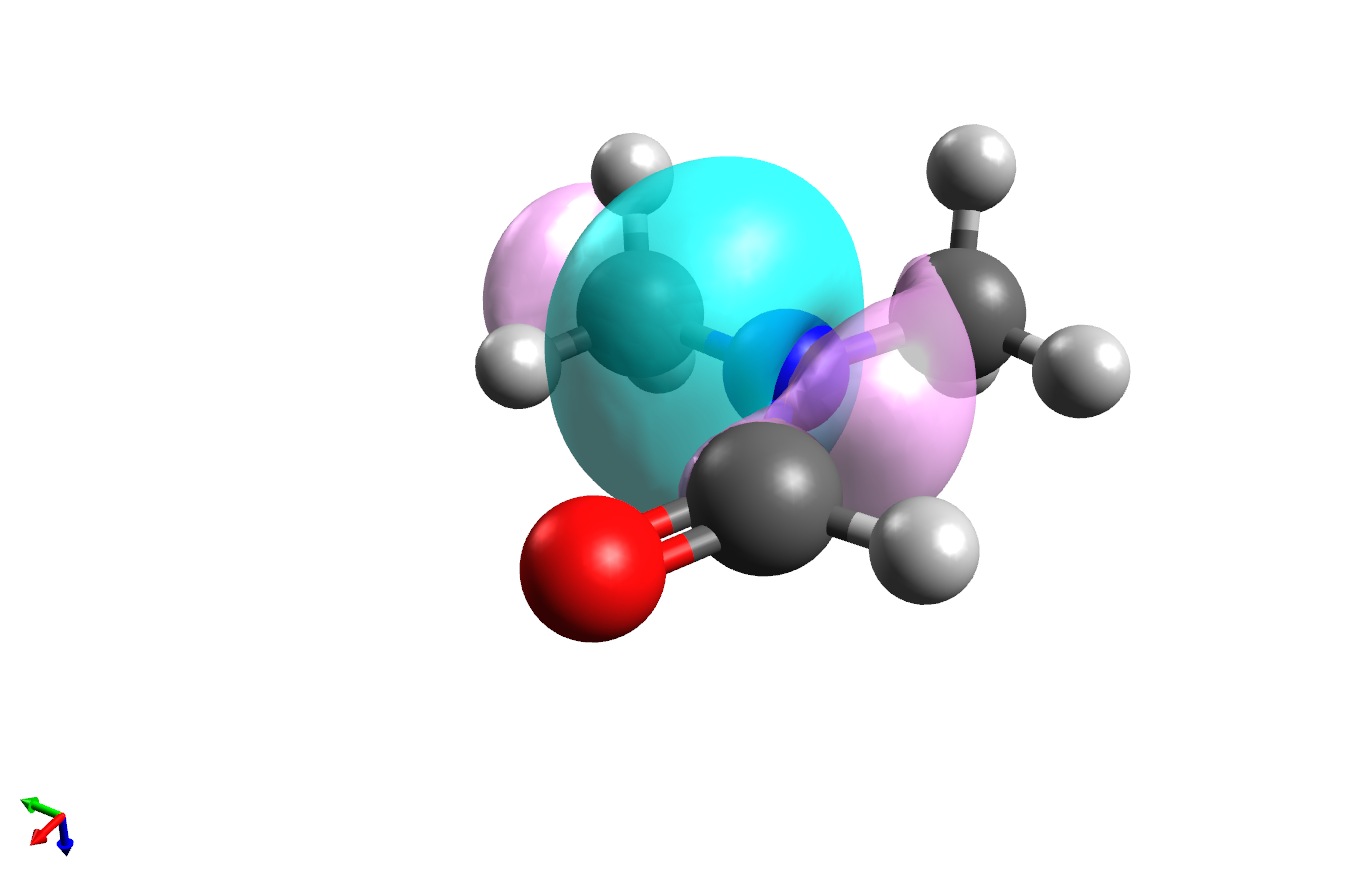
\includegraphics[width=\linewidth]{Figures/dmfnbo-sigma.png}
        \caption{$ \sigma $ bonding NBO.}
    \end{subfigure}
    \begin{subfigure}{0.3\linewidth}
        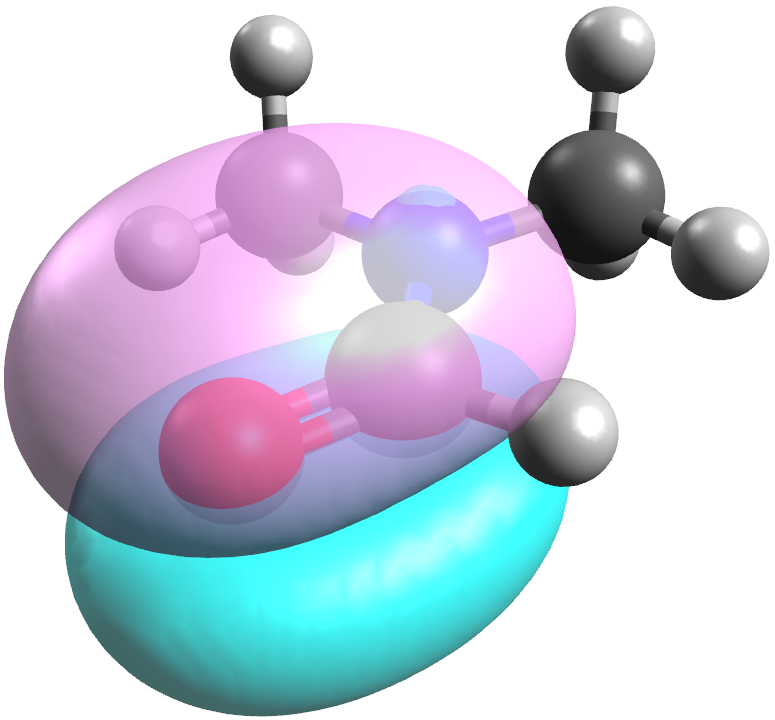
\includegraphics[width=\linewidth]{Figures/dmfnbo-pi.png}
        \caption{$ \pi $ bonding NBO.}
    \end{subfigure}

    \begin{subfigure}{0.3\linewidth}
        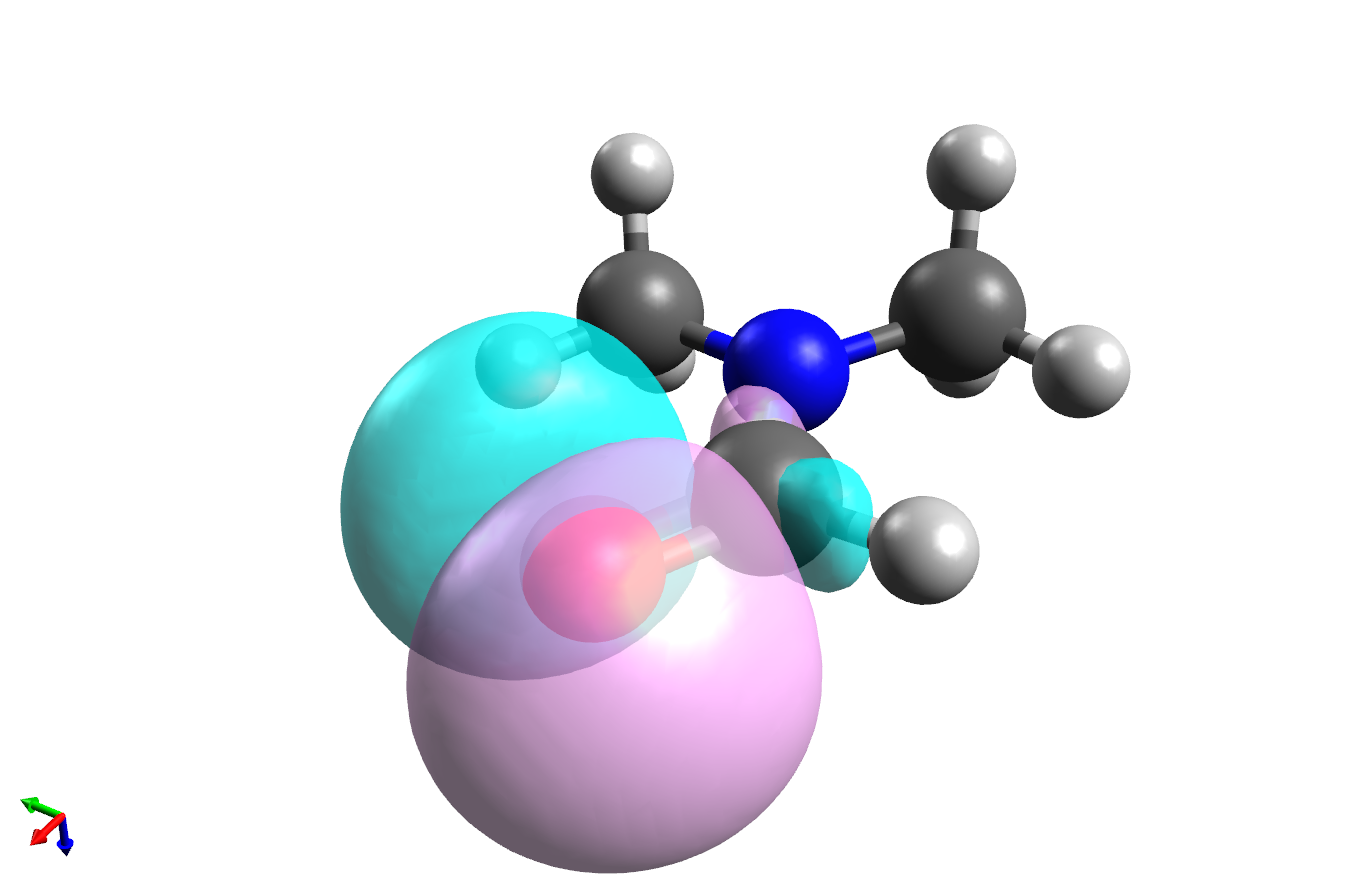
\includegraphics[width=\linewidth]{Figures/dmfnbo-n.png}
        \caption{Lone pair (n) NBO.}
    \end{subfigure}
    \begin{subfigure}{0.3\linewidth}
        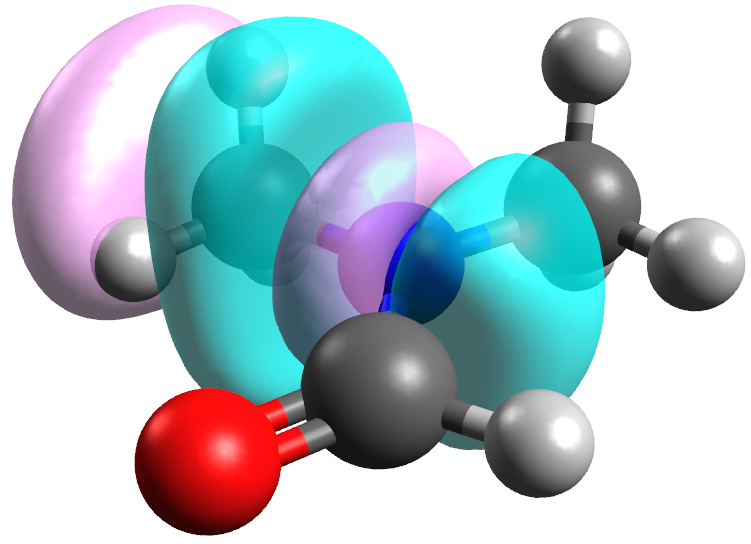
\includegraphics[width=\linewidth]{Figures/dmfnbo-sigmastar.png}
        \caption{$ \sigma^{\star} $ anti-bonding NBO.}
    \end{subfigure}
    \begin{subfigure}{0.3\linewidth}
        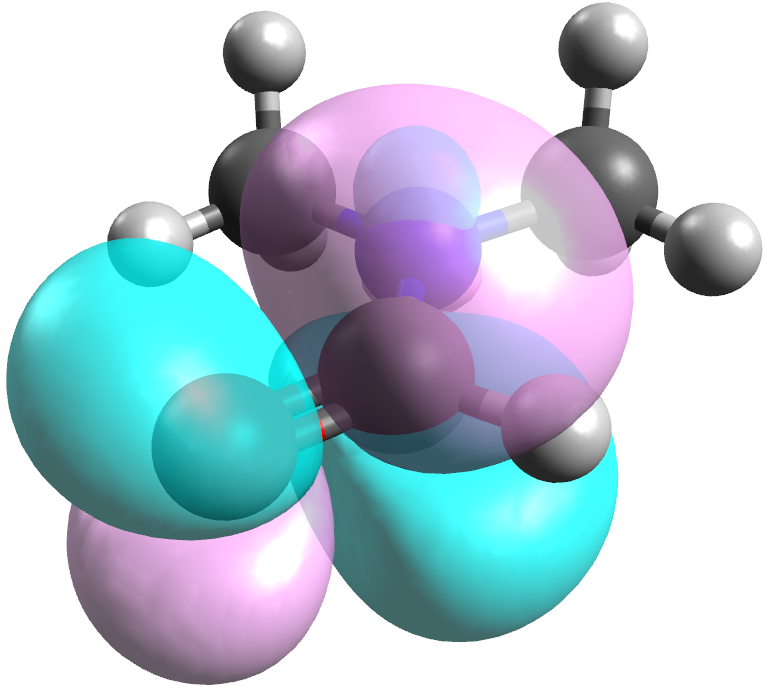
\includegraphics[width=\linewidth]{Figures/dmfnbo-pistar.png}
        \caption{$ \pi^{\star} $ anti-bonding NBO.}
    \end{subfigure}

    \begin{subfigure}{0.3\linewidth}
        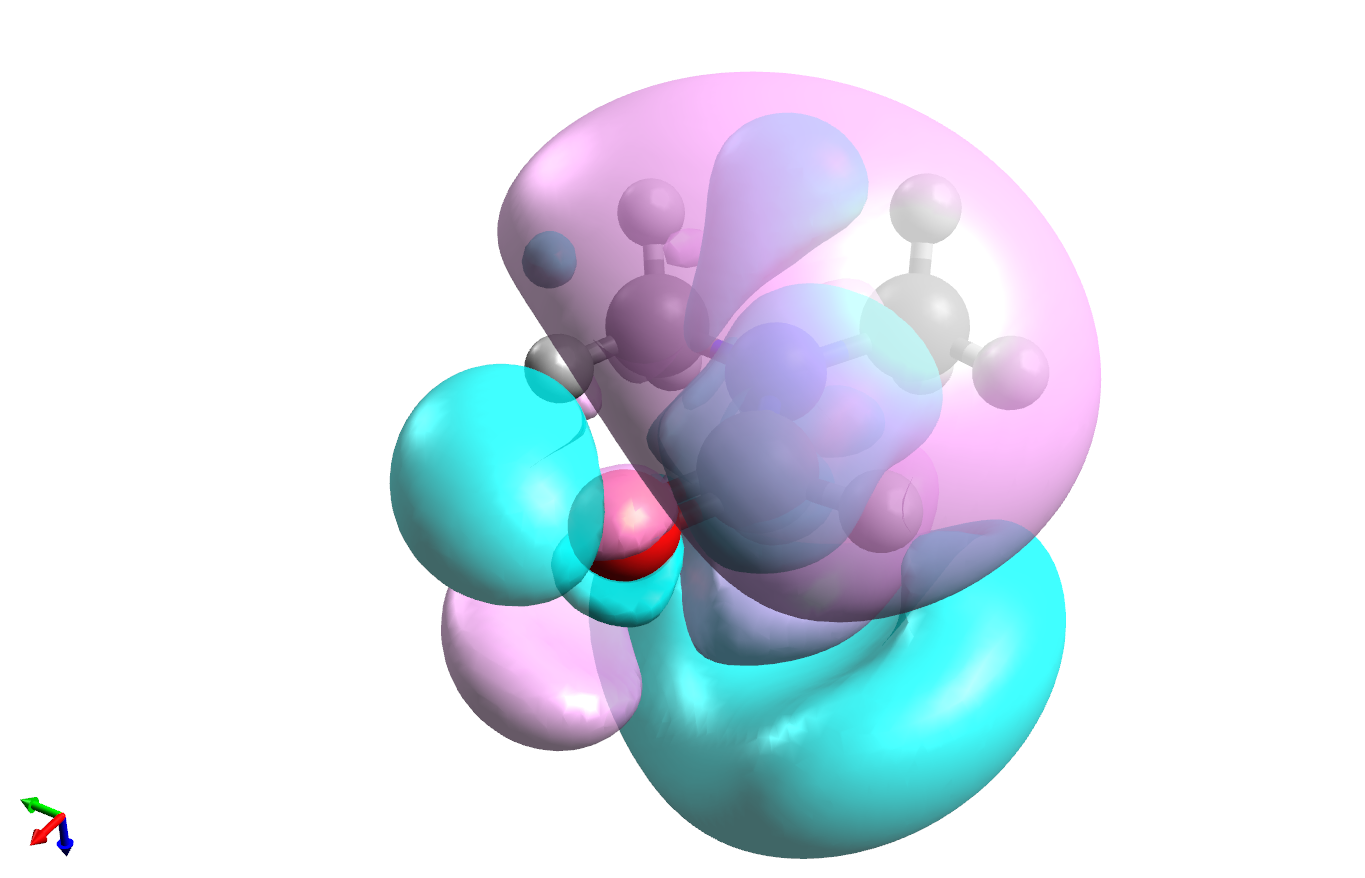
\includegraphics[width=\linewidth]{Figures/dmfnbo-rydberg.png}
        \caption{Rydberg NBO.}
    \end{subfigure}
    \caption{Representative Natural Bond Orbitals of a DMF molecule.}\label{fig:nbos}
\end{figure}

We use NBO theory to rationalise the hyperconjugative effects present in Ch-bonded complexes, namely, the $ \text{n}\rightarrow\sigma^{\star} $ overlap which appears to be present.
NBO analysis allows a numerical value to be assigned to the degree of this overlap, in terms of the formal number of electrons which are ``transferred'' from one orbital to the other.
The energies of each NBO can then be used to calculate the stabilisation afforded by a given delocalisation.

In summary, NBOs are a mathematical transformation of highly delocalised MOs into functions that correspond to the Lewis structure interpretation of chemical bonding.
Although this generates an ideal Lewis structure of a species, departures from this ideal (in the form of delocalisation and hyperconjugative effects) can be seen in decreased occupancy of bonding orbitals and increased occupancy of anti-bonding orbitals.
This allows for a mathematically rigorous and quantitative treatment of bonding, using familiar chemical concepts.

\subsection{Quantum Theory of Atoms In Molecules}\label{sec:qtaim}
The Quantum Theory of Atoms In Molecules (QTAIM) is a description of bonding that is complimentary to that of NBO theory.\autocite{Bader1991}
Rather than describing bonds in terms of orbitals, it uses features of the electron density to define bonding.
This is particularly attractive as orbitals and wave functions are not observable quantities, whereas electron density is.
Indeed electron density can be measured directly through diffraction experiments (see \cref{sec:cd}).
It can also be calculated from a molecular wave function, which can itself be calculated by any number of methods.

To discuss QTAIM, we must first discuss some mathematical aspects of topology.
The fundamental quantity in QTAIM is the electron density $ \rho(\textbf{r}) $, which constitutes a scalar field over the molecule.
That is, every point in space has a single number representing the electron density at that point (see \cref{fig:dmf-rho} for an example).
Differentiating $ \rho(\textbf{r}) $ affords the gradient $ \nabla\rho(\textbf{r}) $, a measure of the local rate of change (in space) of the electron density.
$ \nabla\rho(\textbf{r}) $ is a vector quantity, with a magnitude and direction, which thus forms a vector field.
Differentiating $ \nabla\rho(\textbf{r}) $ again affords the second derivative of $ \rho(\textbf{r}) $, also called the Hessian $ \mathbf{H} $.
$ \mathbf{H} $ is a tensor quantity, which is most commonly represented as a $ 3\times3 $ matrix.
This is not easily represented as a field, but the three eigenvalues (components of the diagonalised Hessian) are useful quantities, which each represent the rate of change of $ \nabla\rho(\textbf{r}) $ at a given point. 
These are given the symbols $ \lambda_1 $, $ \lambda_2 $, and $ \lambda_3 $.
The sum of these eigenvalues is called the Laplacian of the electron density, which is given the symbol $ \nabla^{2}\rho(\textbf{r}) $.
Maps of $ \nabla^{2}\rho(\textbf{r}) $ can recover some chemical features of molecules that are reminiscent of the orbital structure, even though it is derived completely from the $ \rho(\textbf{r}) $ scalar field (\cref{fig:dmf-lapl}).

\begin{figure}
    \centering
    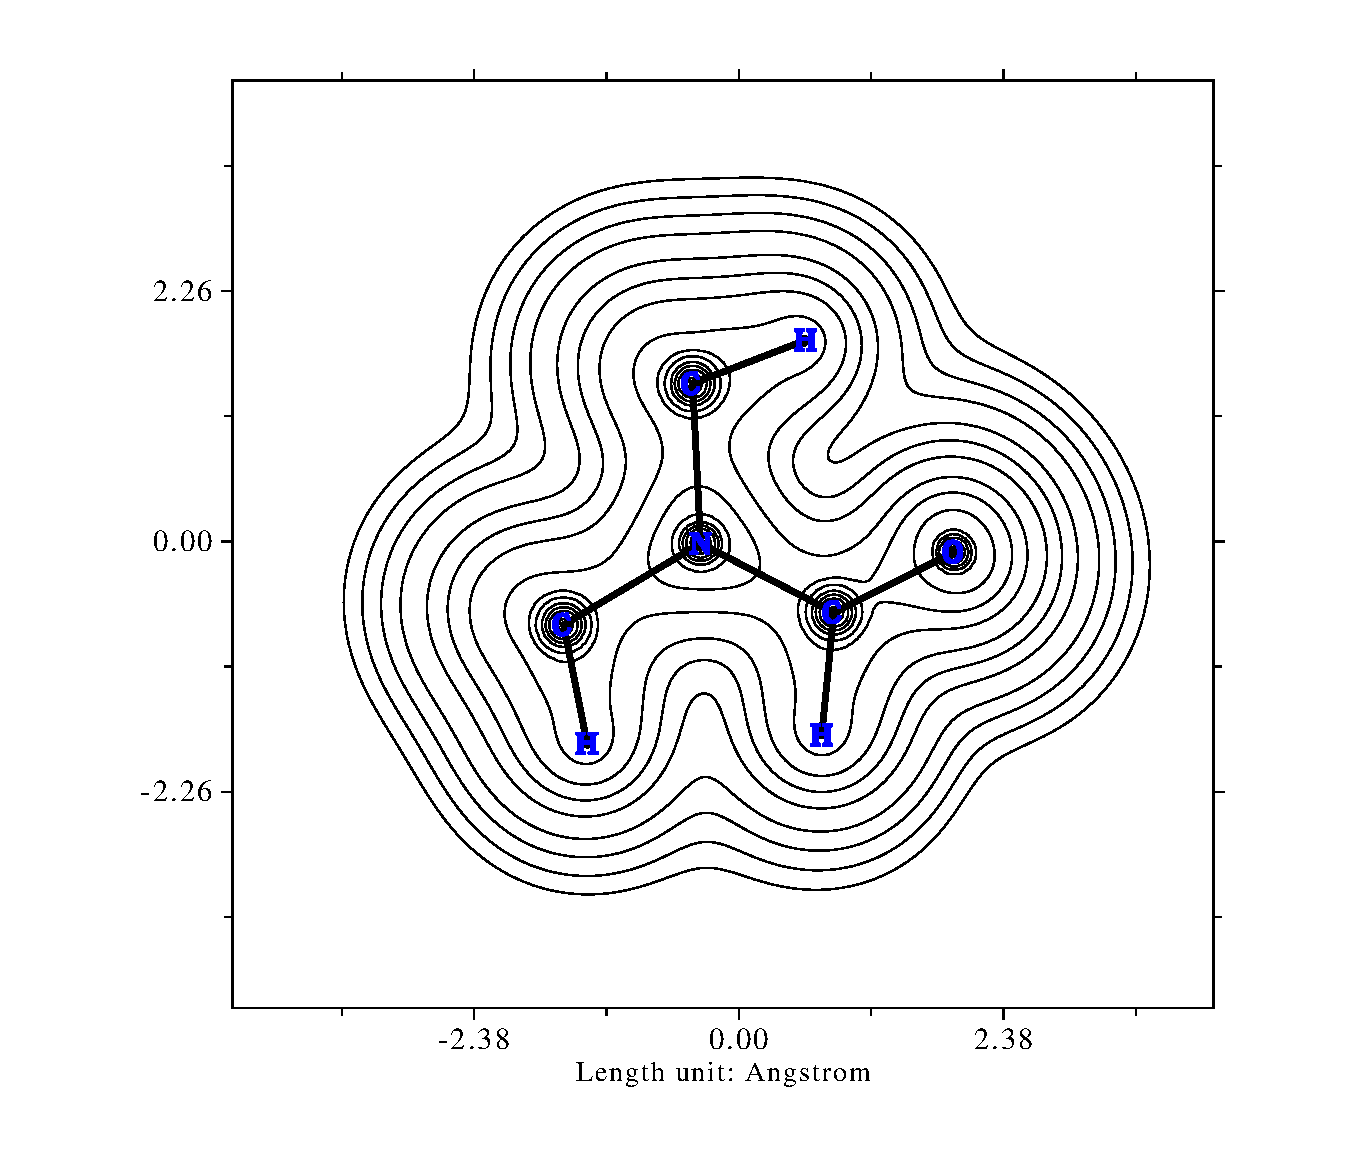
\includegraphics[width=0.48\linewidth]{Figures/dmf-dens-contour.pdf}
    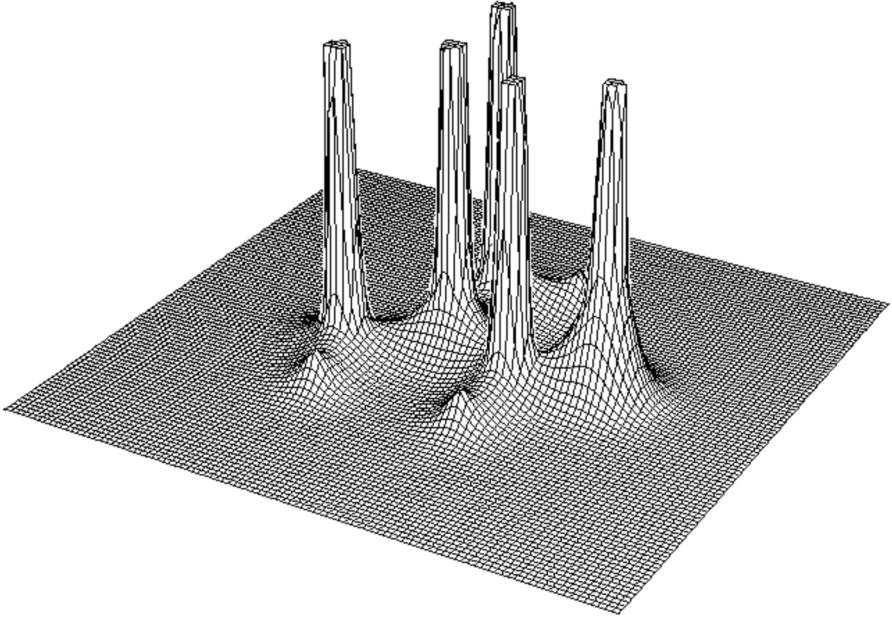
\includegraphics[width=0.48\linewidth]{Figures/dmf-dens-relief.pdf}
    \caption[Electron density $ \rho(\textbf{r}) $ in the plane of a DMF molecule.]{Electron density in the plane of a DMF molecule. The nuclei correspond to the large peaks, and bonds correspond to the ridges linking them.}\label{fig:dmf-rho}
\end{figure}

\begin{figure}
    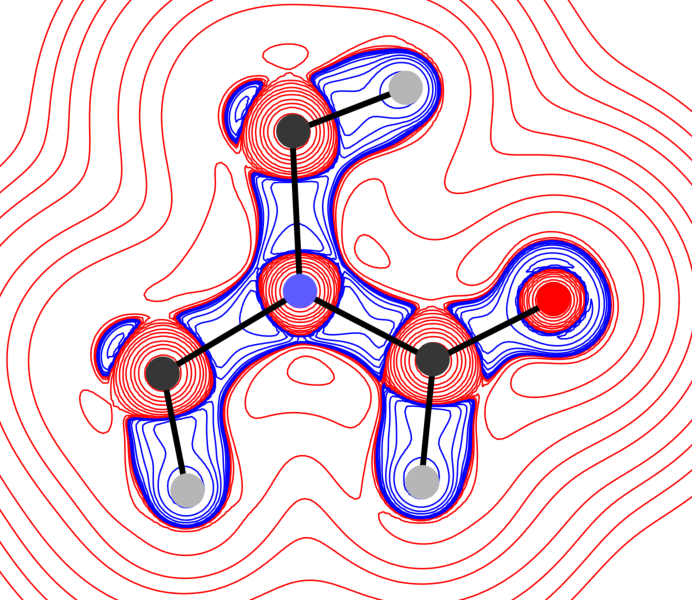
\includegraphics[width=0.48\linewidth]{Figures/dmf-lapl.pdf}
    \caption[Laplacian of the electron density $ \nabla^{2}\rho(\textbf{r}) $ of DMF.]{Laplacian of the electron density $ \nabla^{2}\rho(\textbf{r}) $ of DMF.\@ Positive values are shown in red and negative values in blue. $ \nabla^{2}\rho(\textbf{r}) $ can be seen to recover the shell structure of atoms, as well as chemical features such as bonds and lone pairs.}\label{fig:dmf-lapl}
\end{figure}

A QTAIM atom is defined by a volume bounded by a surface of zero electron density gradient flux (\cref{fig:dmf-gradient}).
That is, there are no field lines of $ \nabla\rho(\textbf{r}) $ crossing the surface.
A molecule can thus be partitioned into atoms, each of which is strictly additive and transferable.
Furthermore, atomic contributions to molecular properties can be uniquely defined.
This is similar to the idea of functional groups in organic chemistry.
In the same way a carboxylic acid functional group can be transferred between molecules while retaining its characteristic properties (its acidity), a QTAIM atom can also be transferred, as its properties depend \emph{only} on the topology of the electron density.

\begin{figure}
    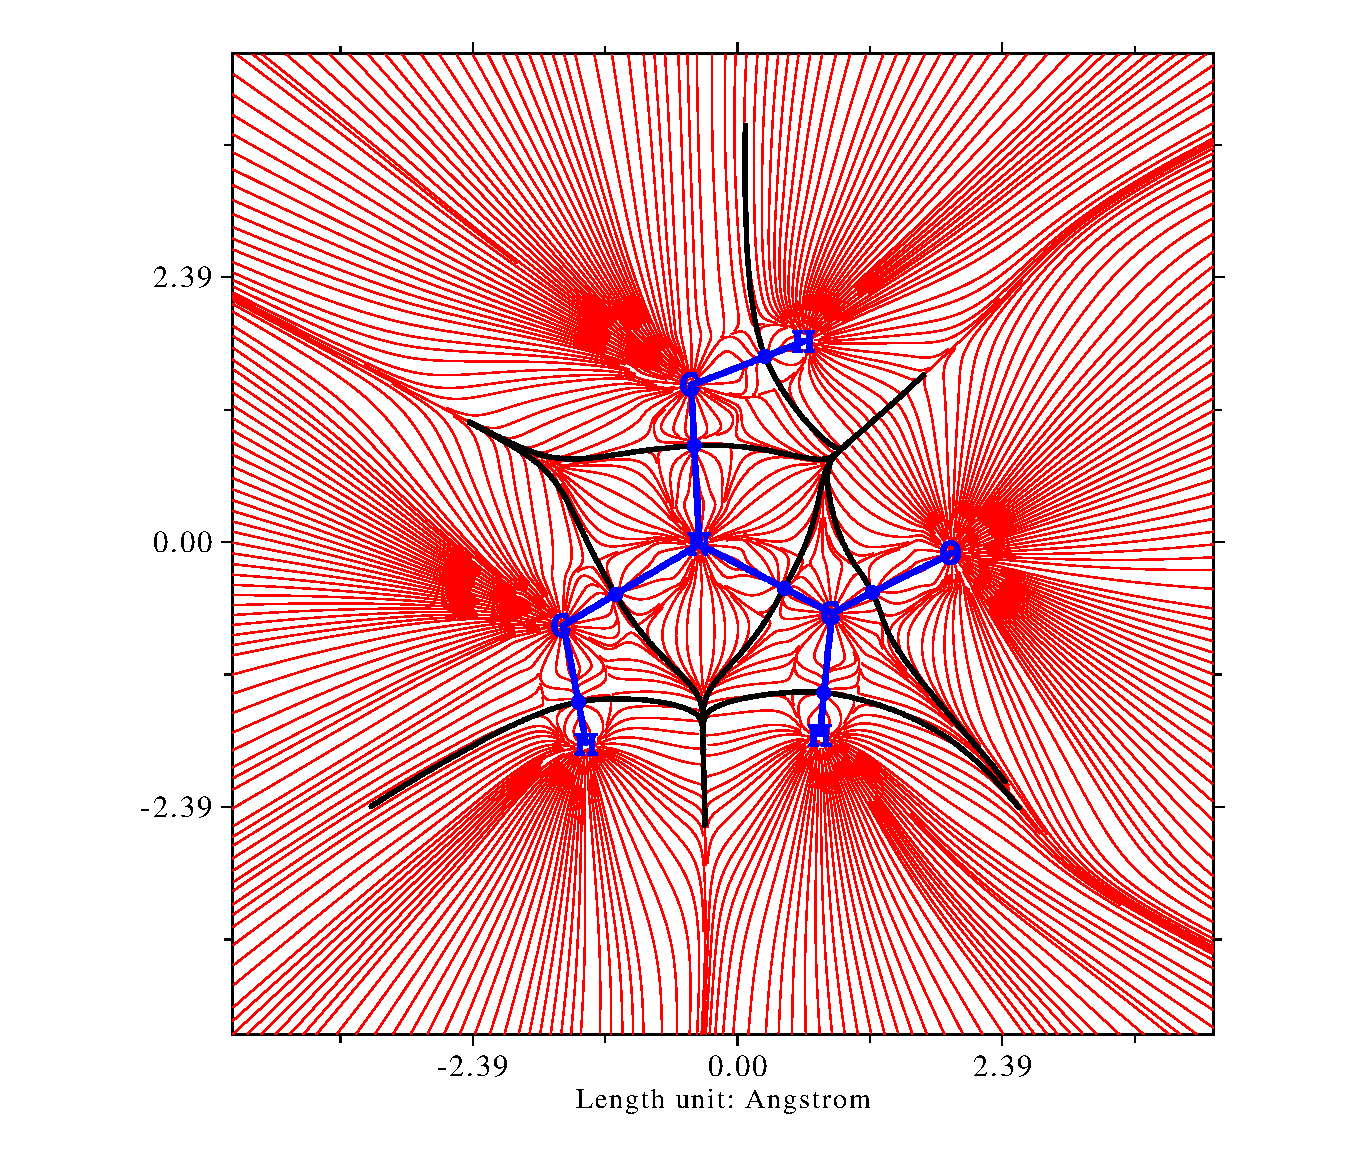
\includegraphics[width=0.48\linewidth]{Figures/dmf-grad.pdf}
    \caption[Electron density gradient $ \nabla\rho(\textbf{r}) $ vector field of DMF.]{Electron density gradient $ \nabla\rho(\textbf{r}) $ vector field of DMF.\@ All field lines (red) converge on the nuclei, and asymptotically approach the zero flux surfaces (black lines) which bound the QTAIM atoms. Bond paths and critical points are shown in blue.}\label{fig:dmf-gradient}
\end{figure}

Each QTAIM atom is associated with a local maximum of electron density which is located at the nucleus.
At this point $ \nabla\rho(\textbf{r}) $ is zero, so it is termed a critical point.
As it is a maximum, $ \rho(\textbf{r}) $ will decrease in all directions, therefore all three eigenvalues of $ \mathbf{H} $ will be negative.
These atomic critical points are therefore termed $ (3,-3) $ critical points, as they exist in three dimensional space and have three negative eigenvalues.

\begin{figure}
    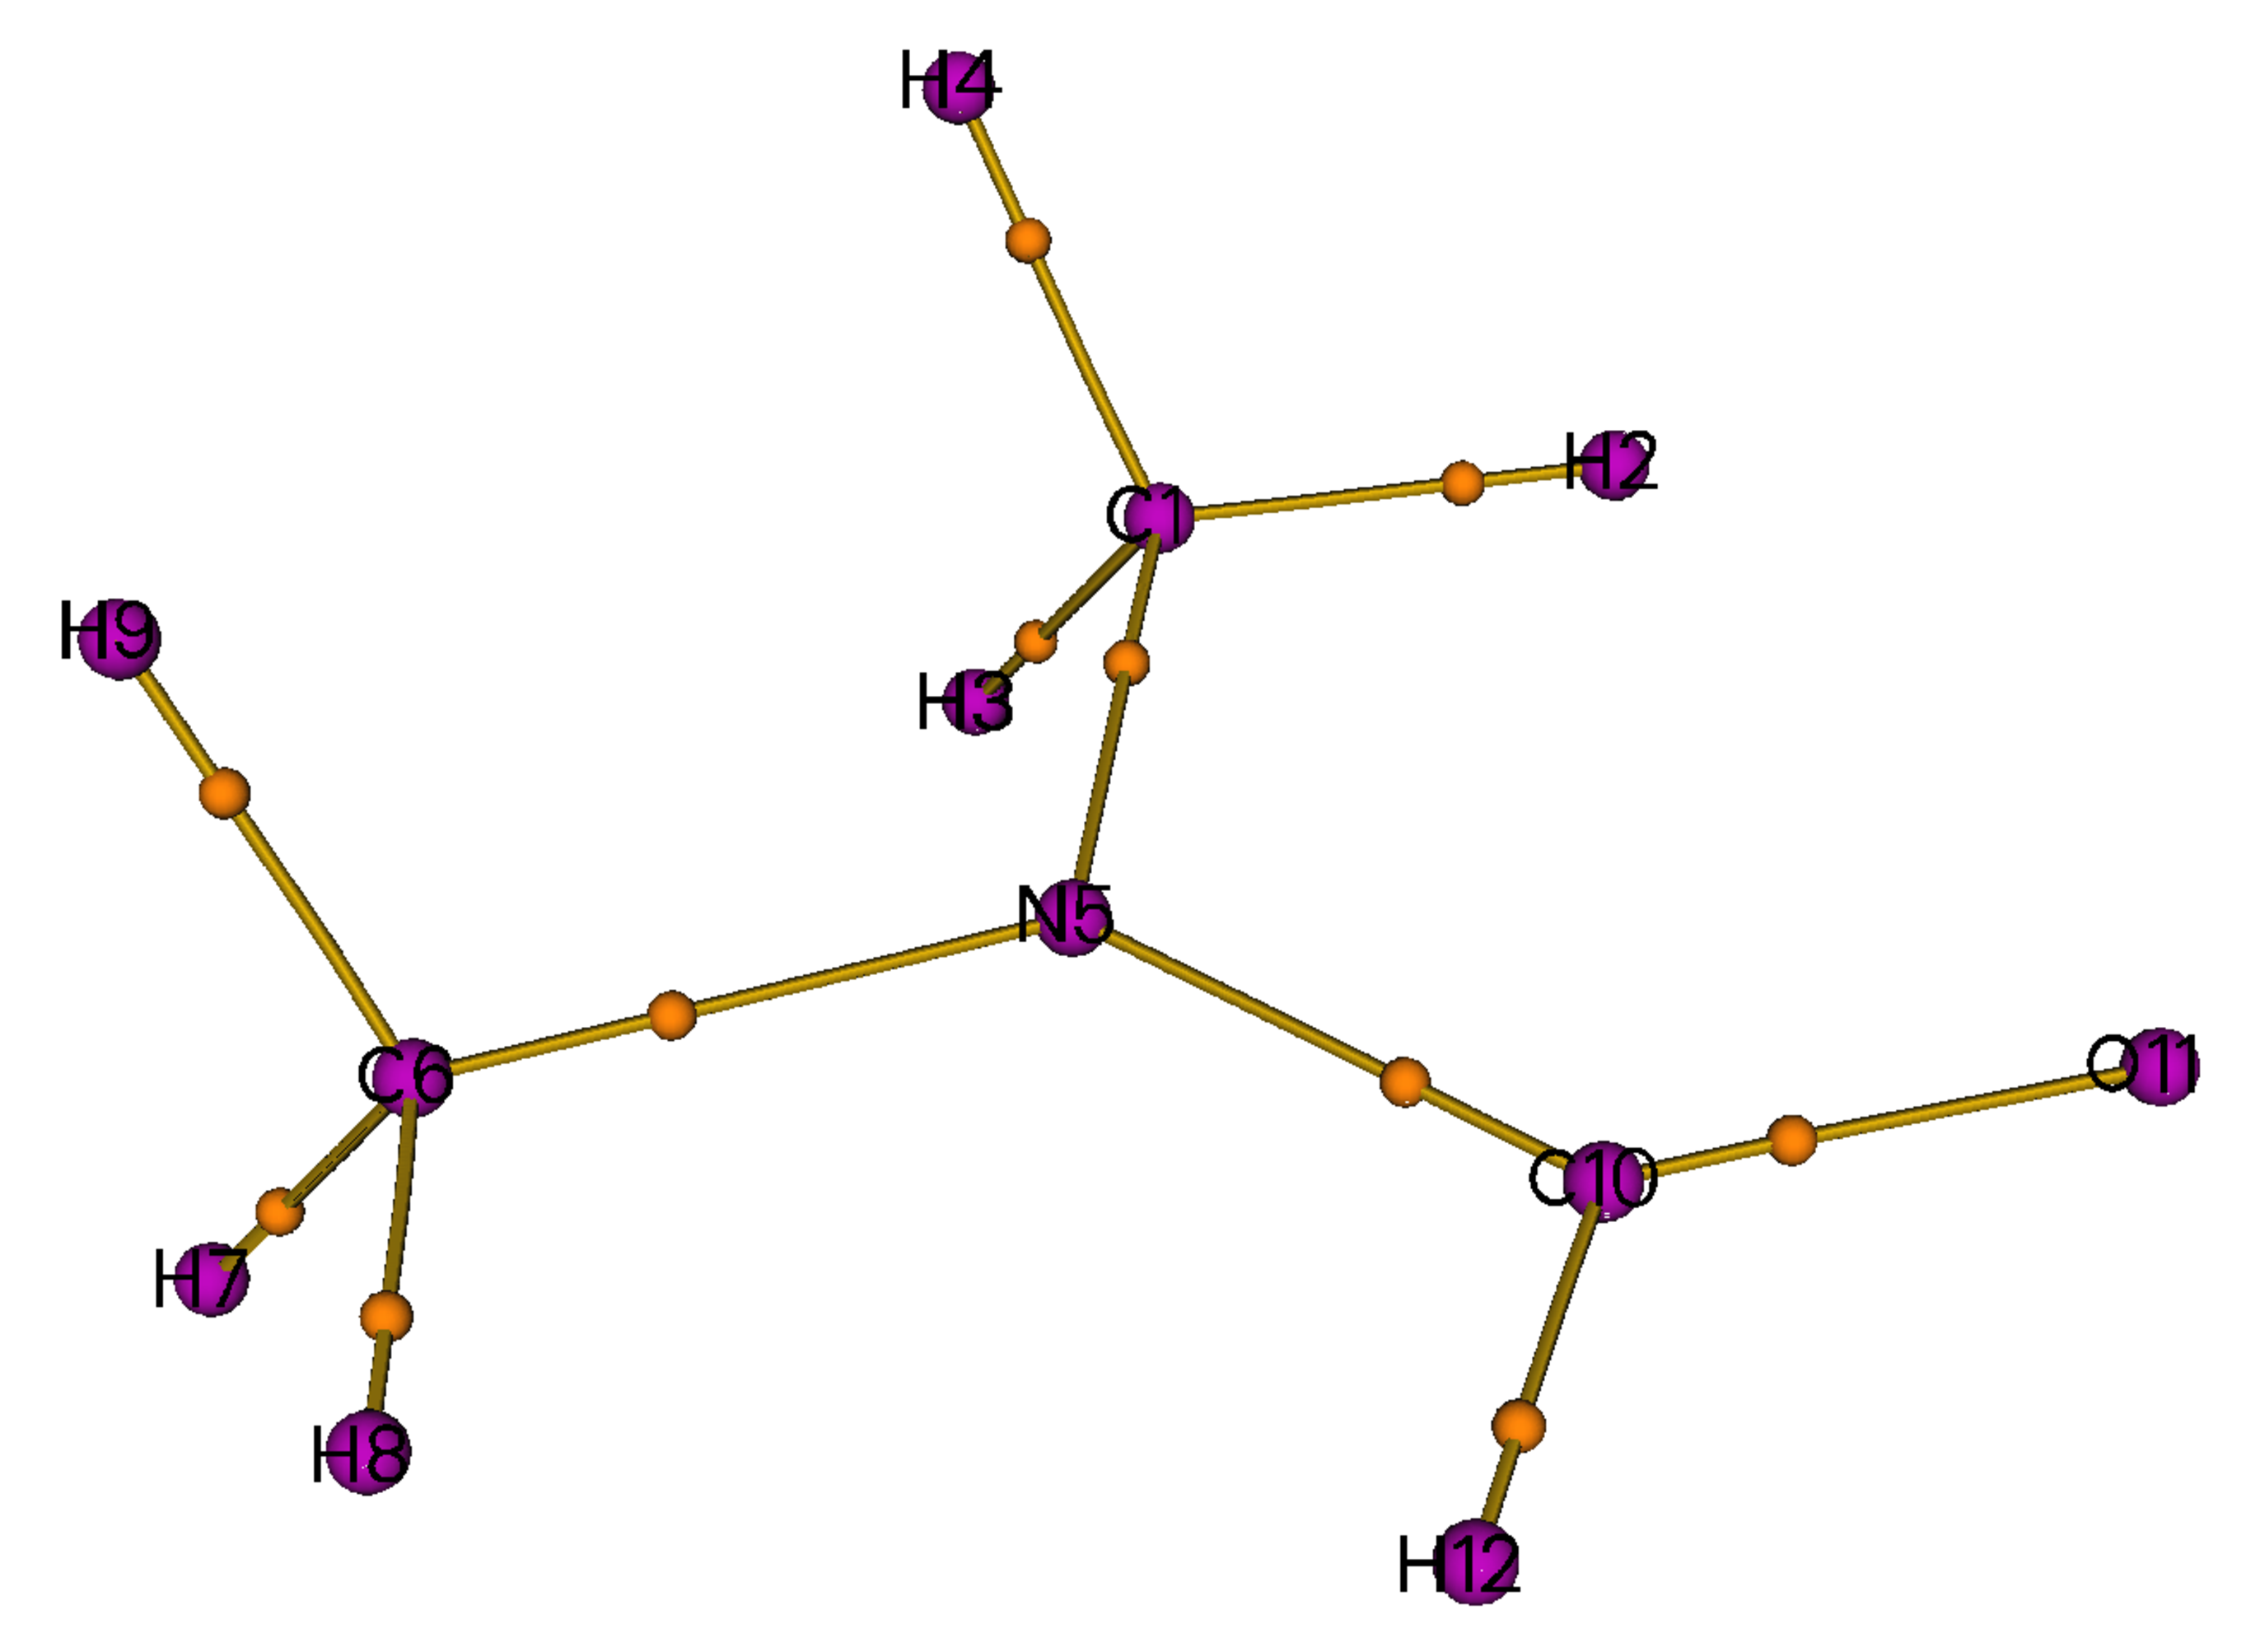
\includegraphics[width=0.45\linewidth]{Figures/dmf-cp.pdf}
    \caption[Critical points of DMF.]{$(3,-3)$ (pink), and $(3,-1)$ (orange) critical points of DMF.\@ Bond paths are shown in yellow.}\label{fig:dmf-cps}
\end{figure}

Nuclei are not the only place critical points are found (where $ \nabla\rho(\textbf{r}) $ is zero).
Atomic critical points contained within neighbouring QTAIM atoms (sharing a common zero gradient flux surface) are linked by lines along which $ \rho(\textbf{r}) $ decreases in the two directions perpendicular to the line.
In two dimensions this can be visualised as a ridge connecting two mountain peaks.
This line is termed a bond path, as the presence of such a line is a prerequisite for bonding to occur (although the reverse is not necessarily true).
At the point where the bond path crosses the zero gradient flux surface there will be another critical point where $ \nabla\rho(\textbf{r}) $ is zero.
This type of critical point is called a bond critical point (BCP) or $ (3,-1) $ critical point, as $ \rho(\textbf{r}) $ decreases in two directions but increases in one direction (along the bond path).
$ \mathbf{H} $ at a $ (3,-1) $ critical point therefore has two negative eigenvalues and one positive eigenvalue.
An example of a molecular structure derived from the critical points and bond paths is shown in \cref{fig:dmf-cps}.
There are also critical points found at the centres of rings (ring or $ (3,1) $ critical points) or at the centres of cage-like structures (cage or $ (3,3) $ critical points), however these are not discussed in this thesis.

As stated before, the presence of a bond path and BCP is necessary but not sufficient to say there is chemical bonding occurring.
In this work we therefore use the presence of a bond path, as measured from experimental electron density, to support our claim that Ch-bonding is occurring.
We also use the values of properties related to $ \rho(\textbf{r}) $ at the BCP to characterise the type of bonding that we observe.
Although this does not replace a proper energy decomposition analysis, certain types of interaction have characteristic values of $ \rho(\textbf{r}) $ and $ \nabla^{2}\rho(\textbf{r}) $ at the BCP.\@ Covalent bonds are characterised by accumulation of electron density between the nuclei, and this is reflected in relatively large values for $ \rho(\textbf{r}) $, and a large and negative value of $ \nabla^{2}\rho(\textbf{r}) $.
Closed shell interactions, on the other hand, do not show this accumulation of charge, so at the BCP $ \rho(\textbf{r}) $ is small, and $ \nabla^{2}\rho(\textbf{r}) $ is positive.

In contrast to NBO theory, QTAIM is a complementary, but equally quantitative and mathematically sound, interpretation of bonding in chemical species.
It has the unique benefit of being grounded solely in the experimentally observable property of the electron density, while still being able to recover chemically intuitive aspects of bonding.

\section{X-ray crystallography}
Single crystal x-ray crystallography is the main experimental technique used in this work.
It allows unambiguous determination of the structure of compounds (including stereochemistry), and  extremely accurate measurement of geometric parameters such as bond lengths.
Practically speaking, a structure is determined by mounting a single crystal of a compound on a goniometer which can rotate the crystal through any orientation, then observing the position and intensity of diffracted x-ray beams.
Rotating the crystal allows different diffraction spots to be observed, and a more complete dataset to be collected.
The position of the diffraction spots provides information about the size and shape of the unit cell, and the intensities provide information about the internal structure i.e.\ the locations of the atoms in the unit cell.
A full discussion of the mathematics of diffraction is outside the scope of this thesis, but the interested reader is referred to \citetitle{Stout1989} by \citeauthor{Stout1989}.\autocite{Stout1989}

\subsection{Charge density refinement}\label{sec:cd}
Fundamental to the technique of x-ray structure determination is the process of refinement, by which parameters of the model (typically the molecular geometry) are optimised to reproduce the observed intensity data as well as possible.
Mathematically, this is performed as a least-squares optimisation, where the function
\begin{equation}
    \sum^{m}_{r=1} w_{r} {\left(F^2_{\mathrm{obs}, r} - F^2_{\mathrm{calc}, r} \right)} ^{2}
\end{equation}
is minimised, where $ F^2_{\mathrm{obs}, r} $ corresponds to the observed intensity, and $ F^2_{\mathrm{calc}, r} $ corresponds to the intensity calculated from the model by Fourier transform.
$ w_{r} $ is a weighting function used to reflect the confidence in any given observed data point.

Assuming the measured intensities are free of any error,\footnote{This is practically never the case, but careful measurement and modern corrections can approach this limit.} this function could theoretically be minimised to zero i.e.\ the model is a complete and true representation of the crystal.
The question then becomes, how do we determine $ F^2_{\mathrm{calc}, r} $ from our model?
To answer this, we must consider what our model actually \emph{is}.

The simplest refinement model consists of atomic coordinates for each atom, plus an overall scale factor (for now we will neglect the anisotropic displacement parameters and chemical occupancies).
However, in order to calculate $ F^2_{\mathrm{calc}, r} $ by Fourier transform, we must introduce some description of what the atoms which we are locating ``look like''.
This forms a hidden, but still crucially important, part of the model.
Typically, atoms are described in reciprocal space as spherically symmetric functions whose contribution to $ F^2_{\mathrm{calc}, r} $ is only dependent on $ (\sin\theta)/\lambda $ (\cref{fig:scatterf}).
This is a consequence of the fact that x-rays are scattered by the \emph{electron cloud} of the atom.\footnote{X-rays have much less energy than the mass-energy of subatomic particles, and so are scattered in the low energy limit of Compton scattering, known as Thompson scattering.
The scattering power of a particle is inversely proportional to the square of its mass, so the massive nuclei contribute negligibly to scattering compared to electrons.}
At $ (\sin\theta)/\lambda = 0 $ the scattering factor is equal to the number of electrons in the atom.
However, the finite size of the electron cloud causes destructive interference and attenuation of the scattering factor as $ (\sin\theta)/\lambda $ increases, as x-rays scattered from one side of the electron cloud will be out of phase with those scattered from the other side.
Contrast this with neutron diffraction, where the neutrons are scattered predominantly by the point-like nucleus, affording a flat scattering function in reciprocal space.
There is almost no destructive interference, and thus neutron crystallography is characterised by an abundance of strong high angle data.
The scattering factor functions for all elements of the periodic table (and many ions) have been calculated based on theoretical electron densities from Hartree-Fock wave functions, and the results are available in the International Tables.\autocite{IntTabCIntensityofdiffractedintensities}
These functions are mercifully incorporated in crystallographic refinement software, shielding them from the user.

\begin{figure}
    \centering
    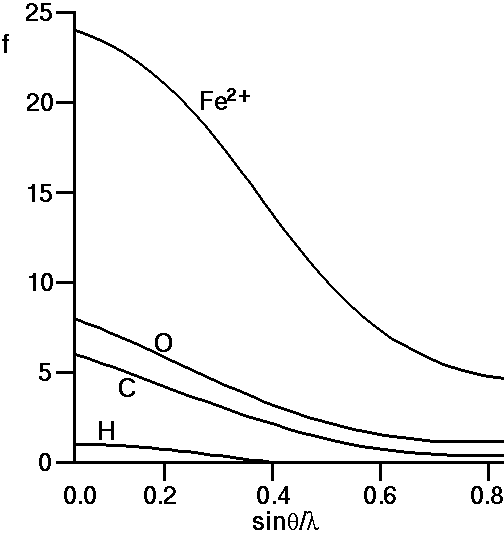
\includegraphics[width=0.5\linewidth]{Figures/scatterf.png}
    \caption{Scattering factors for some atoms as a function of $ (\sin\theta)/\lambda $.}\label{fig:scatterf}
\end{figure}

From the above discussion, one major shortcoming of this approach should be clear.
Namely, that the electron density of bonded atoms is \emph{not} spherically symmetric.
Perturbations such as bonding electron density, lone pairs, and indeed $ \sigma $-holes can, and do, affect the observed scattering factors of atoms, which are not taken into account in typical refinement software.
An extreme case of this, and one that is familiar to any crystallographer, is that of the hydrogen atom.
As the lightest element with only one electron, perturbations due to bonding have an enormous effect, such that the typical \ce{C-H} bond length is underestimated by some 0.13~\AA.\autocite{Cooper2010}
A subtler but more interesting manifestation of this was identified in 1968 by \citeauthor{Coppens1968EvidenceEffects}.\autocite{Coppens1968EvidenceEffects}
X-ray and neutron structures were determined for a crystal of 1,3,5-triazine, and inspection of the difference (a so-called $ \mathrm{X} - \mathrm{N} $ map) revealed unusual systematic variations in the anisotropic displacement parameters.
The nitrogen atoms were deformed radially to the ring, while the carbon atoms were deformed tangentially (\cref{fig:x-n-coppens}).
This is chemically intuitive, as we would expect the lone pairs of the nitrogens to extend radially, while the $ \pi $-electrons of the carbon atoms would form a ring.
The fact that these deformations were incorporated into the anisotropic displacement parameters in the x-ray structure highlights a deficiency of the typical method of refinement.

\begin{figure}
    \centering
    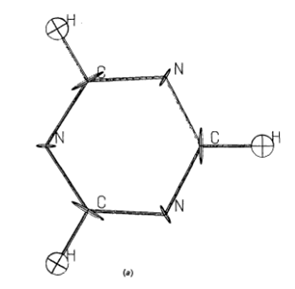
\includegraphics[width=0.5\linewidth]{Figures/x-n-coppens.png}
    \caption[Structure of 1,3,5-triazine.]{$ \mathrm{X} - \mathrm{N} $ map of 1,3,5-triazine, reproduced from \citeauthor{Coppens1968EvidenceEffects}.\autocite{Coppens1968EvidenceEffects}}\label{fig:x-n-coppens}
\end{figure}

Evidence for aspherical atoms can even be traced back to seminal studies performed by \citeauthor{Bragg1920}, in which the famous 222 reflection of a diamond crystal was observed.
The 222 reflection is a systematic extinction of the $ Fd\bar{3}m $ space group to which diamond belongs, but its absence is based on the assumption of spherical atoms.
In diamond, the carbon atoms are actually tetrahedral in form due to the bonding electron density, which lowers the space group symmetry and causes the 222 reflection to be present, though very weak.\autocite{Bragg1920}
Though cutting edge for the time, Bragg's experiment was rather primitive, and multiple scattering likely contributed some intensity to the observed 222 reflection.
The observation was nonetheless correct, and the tetrahedral nature of the carbon atoms in diamond has subsequently been proven time and time again.

Although such perturbations generally only manifest in very high quality structures (aspherical atoms are typically the least of a crystallographer's worries), a number of methods have been proposed to improve refinements, and indeed gain further chemical knowledge from the experimentally determined aspherical electron density.
A simple approach is the use of tabulated aspherical scattering factors for atoms of distinct chemical types.
An example of this is the ELMAM2 database, developed by Jelsch and co-workers.\autocite{Domagaa2012}
The ELMAM2 database consists of experimentally derived scattering factors for all common atom types, with a focus on those found in amino acids and peptides.
A refinement using this database would begin by assigning a type to each atom, which can be done relatively easily using bonding geometries from a more primitive refinement.
This can afford substantial improvement in refinement statistics by providing a more accurate model, at a very modest computational cost.
The obvious drawback of this approach is that the scattering factors must already be tabulated, and the enormous diversity beyond the biochemically important C, H, N, and O precludes the assembly of a truly comprehensive database.
Furthermore, as the scattering factors are pre-tabulated, there is little chemical information that can be extracted from the model beyond somewhat improved precision in geometric parameters.

An improved approach is to compute scattering factors on a case-by-case basis.
This is the rationale behind Hirshfeld Atom Refinement (HARt), first developed by \citeauthor{Jayatilaka2008}.\autocite{Jayatilaka2008}
HARt is an iterative procedure in which the atomic coordinates from a spherical atom refinement (perhaps after correcting \ce{C-H} bond distances) are used to variationally calculate a wave function, from which is calculated an electron density and thus scattering factors.
These new scattering factors improve the model after refinement, from which is calculated a \emph{new} wave function, and so on until the cycles of least squares refinement and wave function calculations converge.
Clearly this repeated calculation of a wave function is computationally expensive, with even relatively simple molecules taking minutes.
Fortunately, however, even very inexpensive levels of theory tend to generate sensible densities for the ground state.
An advantage over the database approach is that one can capture unusual effects in the electron density (such as various non-bonding interaction), provided that they are correctly modelled by the underlying quantum chemistry theory used to generate the wave function.
However this raises a philosophical question: what exactly we are hoping to get out of this procedure?
It can certainly provide improved refinement statistics, including anisotropic refinement of hydrogens in agreement with neutron data, but if we are seeking chemical information about the system, we might as well simply use a gas-phase optimised wave function and dispense with the crystallography.

Related to this is the field of quantum crystallography, which differs somewhat in motivation, if not in methodology.
Quantum crystallography is concerned with extracting a wave function from diffraction data, rather than using a wave function to improve a crystallographic model.
Clearly there is significant overlap.
One method takes inspiration from perturbation theory, where, as in MP2, the Hartree-Fock wave function is taken as the zeroth order approximation.
The diffraction data is then used to construct a perturbative term, which introduces a degree of correlation to the wave function, bringing it closer to the truth (at least within the Born-Oppenheimer approximation).\autocite{Weiss1962}
Even with the power of modern computers, this is not an easy task, and quantum crystallography remains an active and exciting area of research.
It is also worth mentioning the x-ray constrained wave function method developed by \citeauthor{Grimwood2003}.\autocite{Grimwood2003}
This is simply a Hartree-Fock wave function calculation that is constrained via a Lagrangian multiplier to reproduce the observed intensities in the experimental data, assuming there are no crystallographic artifacts in the data such as disorder or twinning.
That is to say, the crystal is simply comprised of infinitely repeating symmetry related molecular units.
The x-ray constrained wave function can be used to calculate a density, which can be used in a HARt-like procedure, which has been named x-ray wave function refinement (XWR).\autocite{Woinska2017}
Both quantum chemistry and crystallographic refinement codes have been implemented in the software package TONTO.\autocite{Jayatilaka2003}

Perhaps the most powerful approach for experimental crystallographers is that of multipole refinement using the formalism developed by Hansen and Coppens.\autocite{Hansen1978}
While superficially similar to quantum crystallographic approaches, no chemical restraint\footnote{This is not strictly true, as electroneutrality is routinely imposed as a constraint on multipole models.} is placed on the resulting electron density, allowing for the modelling of phenomena which are not described by \emph{ab initio} calculations.
The electron density is expanded in a series of atom-centred spherical harmonic basis functions, the local coordinate systems of which are often chosen to align with chemical features.
Each basis function requires two parameters for the occupancy and expansion, in addition to the position and anisotropic displacement parameters for each atom.
We therefore require a large number of observations to ensure the system is overdetermined, and can be treated in a least-squares manner.
Furthermore, the ADPs and dipolar basis terms are highly correlated, leading to an unstable solution if refined simultaneously (\cref{fig:adp-dipole}).

\begin{figure}
    \centering
    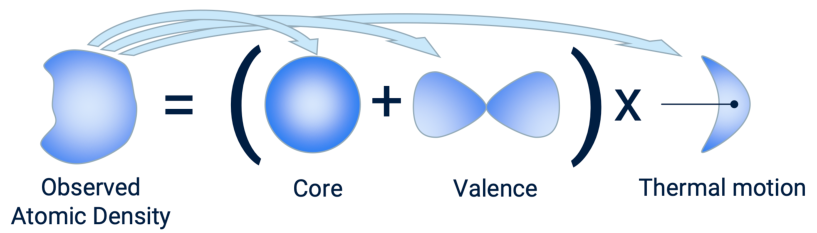
\includegraphics[width=0.6\linewidth]{Figures/valencevsthermaled.pdf}
    \caption[Correlation of thermal and dipolar functions.]{Thermal motion (described by anisotropic displacement parameters) and dipolar basis terms are highly correlated.}\label{fig:adp-dipole}
\end{figure}

For this reason, it is critical to establish accurate atomic positions and ADPs before refining the multipole parameters and charge density.
Traditionally this was done using neutron data which, as mentioned above, is insensitive to electron density perturbations as neutrons are scattered almost exclusively by the nucleus.
Unfortunately neutron sources are notoriously expensive and low-flux, requiring extremely large crystals which introduces further errors due to extinction.
With the advent of modern x-ray diffractometer technology, we can luckily determine atomic coordinates and ADPs using x-ray data alone.
This is done using high angle reflections, which are dominated by core scattering and thus contain little data from the diffuse bonding electron density.
Core electron density is almost perfectly spherical, allowing ADPs to be correctly refined from this data.
With accurate atomic coordinates and ADPs in hand, hydrogen atoms can be located in the low angle data, and then the multipole parameters refined to convergence.
Multipole refinement can benefit enormously from an initial database model, particularly for hydrogen atoms, so it is no surprise that the techniques are often used sequentially.\autocite{Guillot2001,Volkov2006}
The resulting electron density can be used to characterise molecules and predict reactivity, particularly when interpreted within the powerful Quantum Theory of Atoms In Molecules framework of Bader.\autocite{Bader1991}
The obvious attraction of this method is that it is almost entirely experimental.
However, the atom centred multipole functions and their resulting sum, while superficially resembling a wave function, is not antisymmetric and is therefore in violation of the Pauli exclusion principle.
It therefore cannot be used to determine \emph{all} properties of a system.

To summarise, electron density can be measured in a crystal by x-ray diffraction, and various models used to fit it.
The ``gold standard'' would be the derivation of a wave function, but at present this has not been done without the introduction of chemical constraints.
In practise, the most accurate and most informative fitting of electron density to diffraction data is done with a series of atom-centred spherical harmonic functions (the Hansen-Coppens formalism).
The resulting electron density can be used in QTAIM analysis, or used to construct electrostatic potential maps, which can guide chemists in their understanding of molecules in crystals.

\section{Nuclear Magnetic Resonance}
Nuclear magnetic resonance spectroscopy (NMR) is an essential tool for all organic chemists, as it is able to give relatively detailed structural information quickly and cheaply.
It is based on the magnetic moment of certain nuclei, which are usually randomly oriented but spontaneously align in the presence of a strong magnetic field.

\subsection{Solid State NMR}
The chemical shift of a nucleus is not a simple scalar quantity, as solution phase NMR experiments might suggest.
The shielding, and hence the effective magnetic field felt by the nucleus depends on the electronic environment around the nucleus, which is decidedly \emph{an}isotropic, therefore incapable of being expressed as a scalar.
Depending on the orientation of the electron cloud (and other shielding/deshielding influences) around the nucleus with respect to the magnetic field, different chemical shifts will be observed for the same nucleus.
This phenomenon is the chemical shift anisotropy of a nucleus, and it is described mathematically by a second rank tensor, which is geometrically depicted as an ellipsoid.

In a solution phase NMR experiment, rapid and random tumbling of the molecules averages out the anisotropy of each signal, affording a sharp peak at the isotropic chemical shift.
This can be simulated to some degree by magic angle spinning in solid-state experiments, but it is often the case that the chemical shift anisotropy is more interesting that the isotropic shift, so a solid phase NMR experiment is the only way to examine it.

The shape of the chemical shift tensor can provide insight into the electronic environment of a nucleus, with large shielding components often being aligned with electronic features such as bonds or lone pairs.
It is often convenient to define a principal axis system (PAS) for the tensor, consisting of two components which describe the longest and shortest axes of the ellipsoid, and the axis perpendicular to both.
The PAS of the chemical shielding tensor is denoted by the lowercase $ x $, $ y $ and $ z $, and the components of the tensor which are aligned with these axes are labelled $ \sigma_{xx} $, $ \sigma_{yy} $ and $ \sigma_{zz} $.
The laboratory reference frame is denoted by the uppercase $ X $, $ Y $ and $ Z $, with the magnetic field $ B_0 $ being aligned with the $ Z $ axis.
A common method for transforming one coordinate system to another is through the use of Euler angles $ \alpha $, $ \beta $ and $ \gamma $, which define sequential right-handed rotations about the axes of the rotating frame.
As the chemical shielding is necessarily invariant to rotation about $ Z $, we can dispense with the first of these angles $ \alpha $, and simply refer to the latter two as the polar angles $ \beta = \theta $ and $ \gamma = \phi $.
The chemical shielding tensor is thus depicted in \cref{fig:chemical-shielding-tensor}, and this will be the convention used in this work.

\begin{figure}
  \centering
  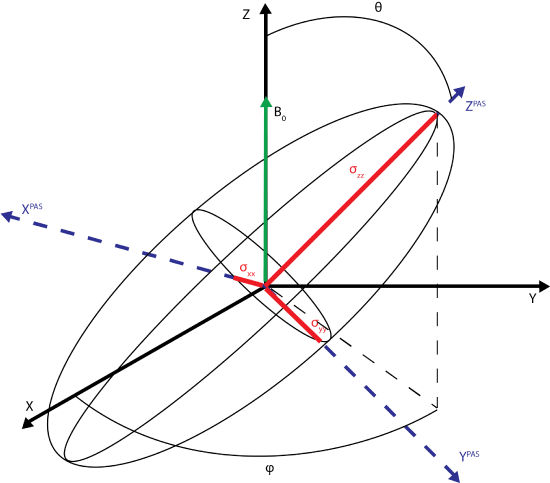
\includegraphics[width=0.4\linewidth]{Figures/Chemical_Shift_Tensor.png}
  \caption[Principal axis system with respect to laboratory reference.]{Representation of the principal axis system (PAS, blue dotted lines) with respect to the laboratory reference frame (black solid lines). The polar angles $ \theta $ and $ \phi $ relate the former to the latter. The principal components of the tensor are shown in red, and the overall shape is shown by the black ellipses.}\label{fig:chemical-shielding-tensor}
\end{figure}

In almost all experiments, the chemical shielding tensor $ \sigma $ is only indirectly measured, via the chemical shift $ \delta $, which is defined with respect to a reference nucleus such that $ \delta = \sigma_{\textrm{ref}} - \sigma_{\textrm{sample}} $.
As the coordinate system as described above is somewhat arbitrary, the IUPAC convention defines the three principal components of the chemical shift tensor $ \delta_{11} $, $ \delta_{22} $ and $ \delta_{33} $ such that $ \delta_{11} \geq \delta_{22} \geq \delta_{33} $.
The isotropic chemical shift is given by the average $ \delta_{\textrm{iso}} = \frac{(\delta_{11} + \delta_{22} + \delta_{33})}{3} $.
There are two other conventions for describing chemical shift anisotropy, which are useful in different contexts.
The Herzfeld Berger convention represents the chemical shift in terms of the span of the signal $ \Omega = \delta_{11} - \delta_{33} $ and the skew $ \kappa = \frac{3(\delta_{22} - \delta_{\textrm{iso}})}{\Omega} $ where $ \delta_{\textrm{iso}} $ is the same as in the IUPAC convention.
This is particularly useful for intuitively describing the powder line shape formed by a given signal.
The other convention is the Haeberlen convention, which defines the three principal components as $ |\delta_{zz} - \delta_{\textrm{iso}}| \geq |\delta_{xx} - \delta_{\textrm{iso}}| \geq |\delta_{yy} - \delta_{\textrm{iso}}| $, and the parameters $ \Delta_{\textrm{CSA}} = \delta_{zz} -\delta_{\textrm{iso}} $ and $ \eta_{\textrm{CSA}} = \frac{\delta_{xx} - \delta_{yy}}{\delta_{zz} -\delta_{\textrm{iso}}} $.
This convention is most useful for describing the angular dependence of a chemical shift on the polar angles $ \theta $ and $ \phi $, which is given by the relationship\autocite{Haeberlen1976}
\begin{equation}
  \delta_{\textrm{obs}} = \delta_{\textrm{iso}} + \Delta_{\textrm{CSA}} \left(\frac{3 \cos^2 \theta - 1 + \eta_{\textrm{CSA}} \sin^2 \theta \cos 2 \phi}{2} \right)
  \label{eqn:orientation-csa}
\end{equation}

In a non-spinning polycrystalline or amorphous powder, the above expression can be integrated over the range of chemical shifts to give the characteristic powder line shape see in \cref{fig:ssnmr-tensor}, reproduced from the work of Facelli, Grant, and Michl.\autocite{Facelli1987Carbon-13Determination}
The sample consists of randomly oriented tensors, all of which contribute to the signal.
The principal values of the tensor $ \delta_{11} $, $ \delta_{22} $ and $ \delta_{33} $ correspond to the two extrema of the line, and the central peak.

\begin{figure}
  \centering
  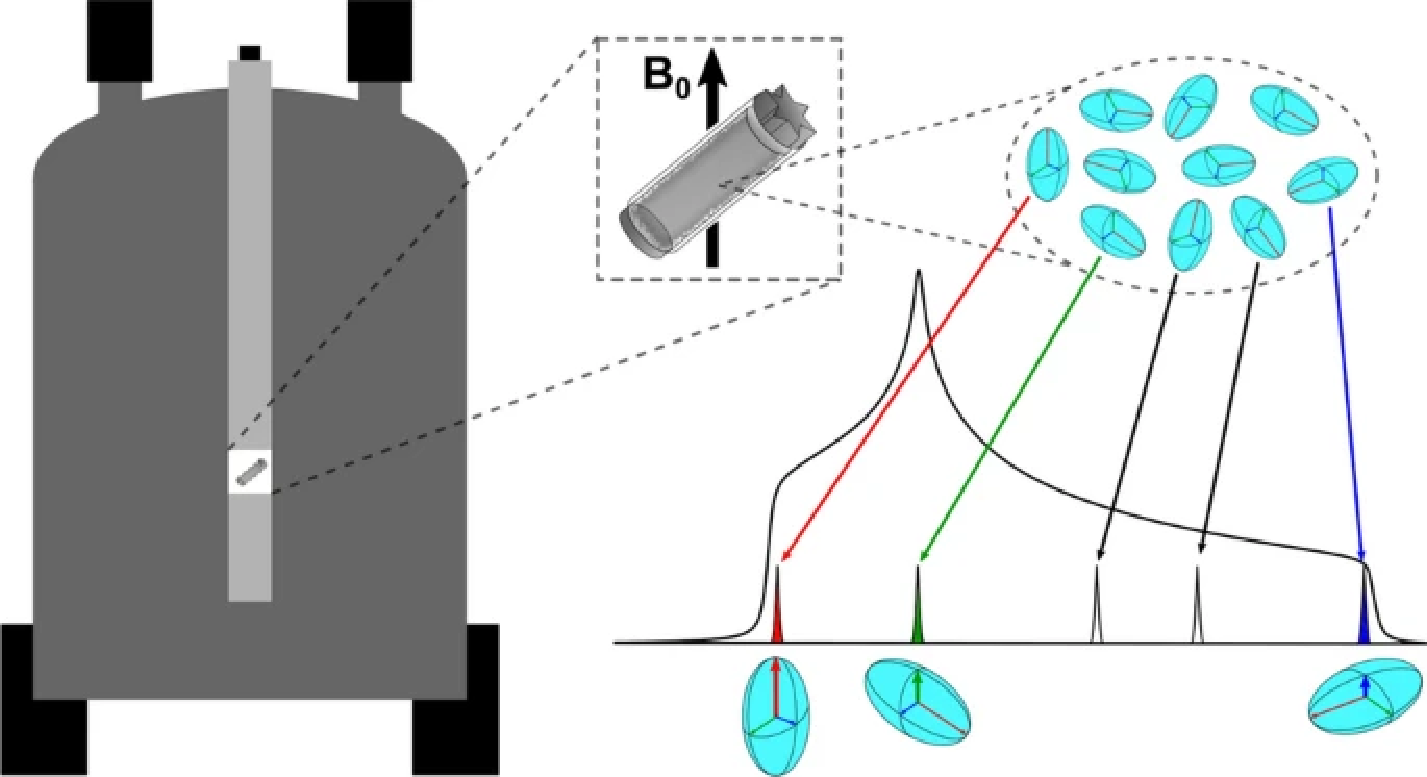
\includegraphics[width=0.45\linewidth]{Figures/ssnmr-tensor.pdf}
  \caption[SS-NMR powder line shape.]{Characteristic solid-state NMR powder line shape for an asymmetric tensor e.g.\ in an alkene. The positions of the three principal values are shown.}\label{fig:ssnmr-tensor}
\end{figure}

Spinning at the magic angle can improve the S/N ratio by partially averaging out the chemical shift anisotropy and dipolar relaxation.
Instead of the powder pattern, we instead observe a sharp isotropic chemical shift and a series of spinning sidebands which are separated from the isotropic peak by multiples of the spinning frequency.
The radiated power is thus concentrated in narrower bands, leading to a much improved S/N ratio.

An example is presented in \cref{fig:31P-ssnmr} of proton decoupled solid state \ce{^{31}P} spectra of barium diethyl phosphate, reproduced from the work of Herzfeld and Berger\autocite{Herzfeld1980SidebandAngle}.
In the first spectrum, no magic angle spinning was used, and the line shape is characteristically broadened into an asymmetric peak (the powder line shape).
Note the poor S/N ratio due to the broad peak.
The S/N ratio can be seen to improve as the spinning speed increases, and the sidebands become more sparse, affording a stronger signal overall.

\begin{figure}
    \centering
    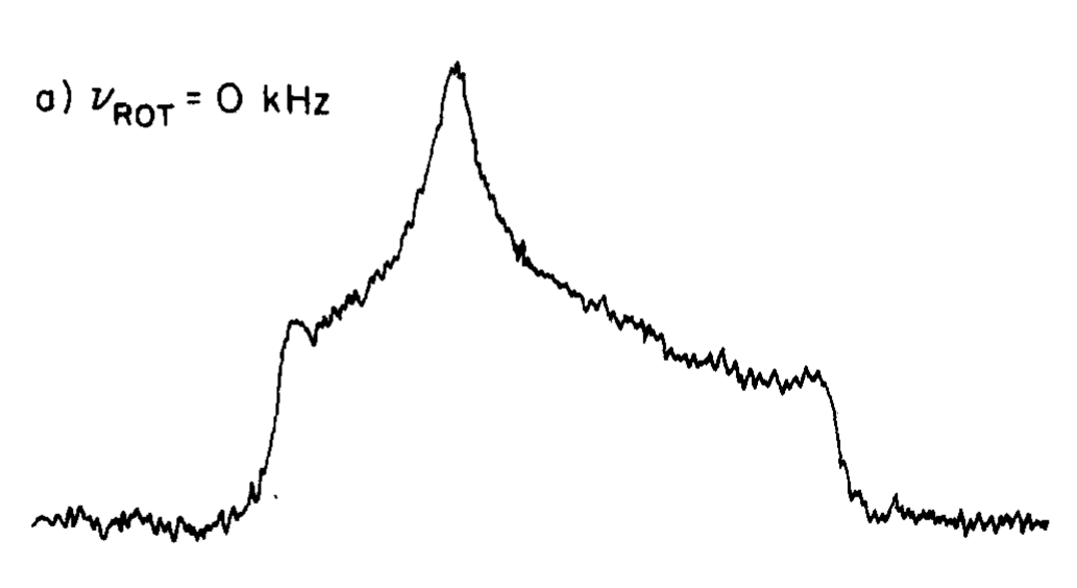
\includegraphics[width=0.45\linewidth]{Figures/31P-ssnmr-0khz.pdf}
    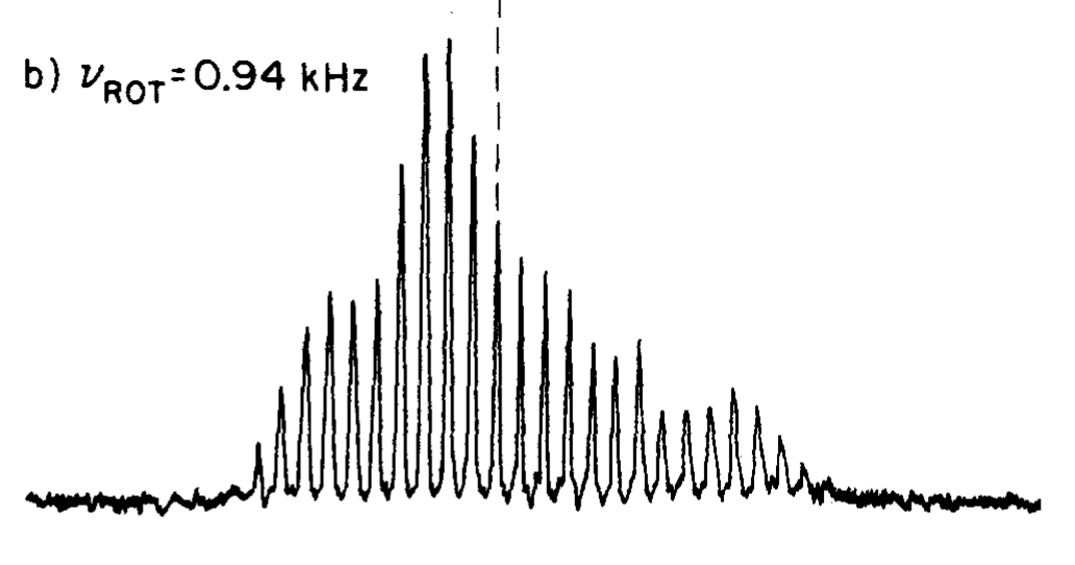
\includegraphics[width=0.45\linewidth]{Figures/31P-ssnmr-0.94khz.pdf}

    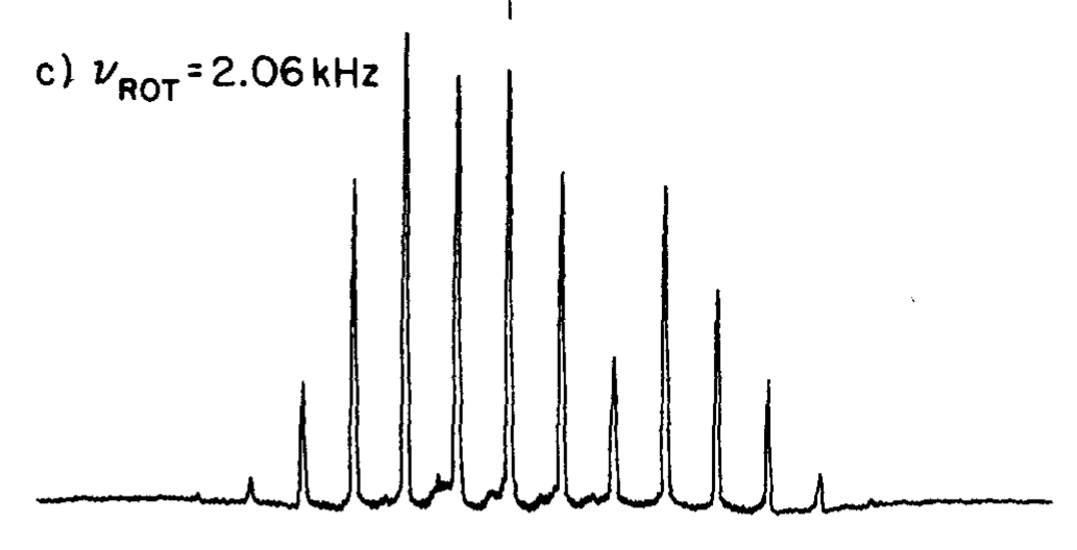
\includegraphics[width=0.45\linewidth]{Figures/31P-ssnmr-2.06khz.pdf}
    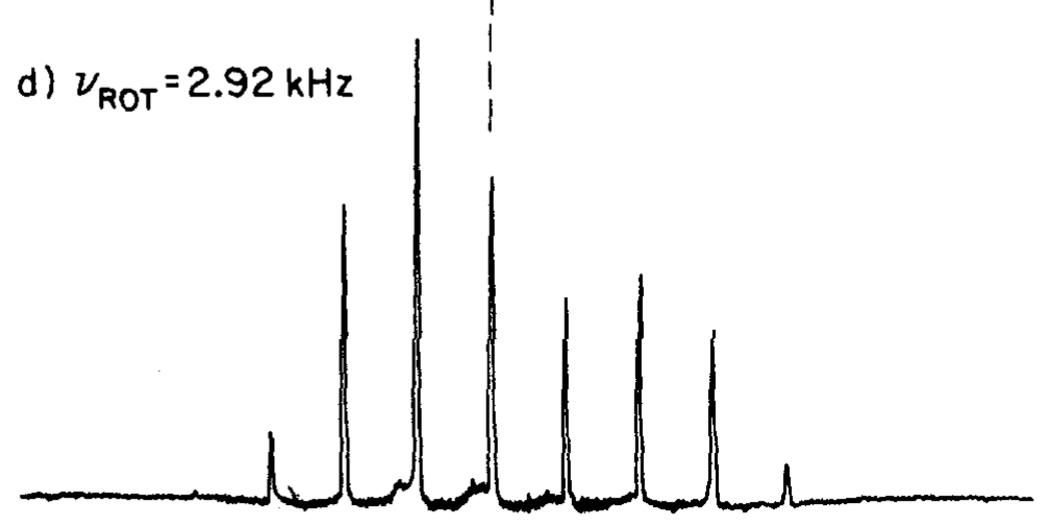
\includegraphics[width=0.45\linewidth]{Figures/31P-ssnmr-2.92khz.pdf}
    \caption[\ce{^{31}P}-SS-NMR spinning at the magic angle.]{Proton decoupled solid state \ce{^{31}P} spectra of barium diethyl phosphate spinning at the magic angle, at the speed specified. The isotropic chemical shift is shown by the vertical dotted line.}\label{fig:31P-ssnmr}
\end{figure}

The principal values of the tensor are clearly easily obtained from a non-spinning sample, as they can practically be read off the spectrum.
However, the extremely poor S/N ratio (especially for a relatively insensitive nucleus like \ce{^{77}Se}) limits the utility of this method.
Spinning at the magic angle is clearly necessary to improve the S/N ratio, however this obscures the true locations of the extrema of the signal, therefore the values of $ \delta_{11} $ and $ \delta_{33} $, as well as modifying the position of the maximum ($ \delta_{22} $).

There exist programs (such as SOLA, integrated within TopSpin by Bruker BioSpin) which can fit an experimental line shape or sideband manifold affording the principal values of the tensor, however there is clearly a trade-off between obtaining a good S/N ratio and having enough sidebands within the limits of the signal for a meaningful fit.
Perhaps the most fundamental issue stems from the fact that the sample is a powder of randomly oriented particles.
This means that the absolute orientation of the tensor with respect to the molecule cannot be determined from this kind of experiment.
Nonetheless, the \emph{shape} of the tensor is still valuable information that may be able to shed light on Ch-bonding in the solid phase.

\printbibliography[heading=subbibliography]
\end{refsection}
